% Template for PLoS
% Version 3.1 February 2015
%
% To compile to pdf, run:
% latex plos.template
% bibtex plos.template
% latex plos.template
% latex plos.template
% dvipdf plos.template
%
% % % % % % % % % % % % % % % % % % % % % %
%
% -- IMPORTANT NOTE
%
% This template contains comments intended 
% to minimize problems and delays during our production 
% process. Please follow the template instructions
% whenever possible.
%
% % % % % % % % % % % % % % % % % % % % % % % 
%
% Once your paper is accepted for publication, 
% PLEASE REMOVE ALL TRACKED CHANGES in this file and leave only
% the final text of your manuscript.
%
% There are no restrictions on package use within the LaTeX files except that 
% no packages listed in the template may be deleted.
%
% Please do not include colors or graphics in the text.
%
% Please do not create a heading level below \subsection. For 3rd level headings, use \paragraph{}.
%
% % % % % % % % % % % % % % % % % % % % % % %
%
% -- FIGURES AND TABLES
%
% Please include tables/figure captions directly after the paragraph where they are first cited in the text.
%
% DO NOT INCLUDE GRAPHICS IN YOUR MANUSCRIPT
% - Figures should be uploaded separately from your manuscript file. 
% - Figures generated using LaTeX should be extracted and removed from the PDF before submission. 
% - Figures containing multiple panels/subfigures must be combined into one image file before submission.
% For figure citations, please use "Fig." instead of "Figure".
% See http://www.plosone.org/static/figureGuidelines for PLOS figure guidelines.
%
% Tables should be cell-based and may not contain:
% - tabs/spacing/line breaks within cells to alter layout or alignment
% - vertically-merged cells (no tabular environments within tabular environments, do not use \multirow)
% - colors, shading, or graphic objects
% See http://www.plosone.org/static/figureGuidelines#tables for table guidelines.
%
% For tables that exceed the width of the text column, use the adjustwidth environment as illustrated in the example table in text below.
%
% % % % % % % % % % % % % % % % % % % % % % % %
%
% -- EQUATIONS, MATH SYMBOLS, SUBSCRIPTS, AND SUPERSCRIPTS
%
% IMPORTANT
% Below are a few tips to help format your equations and other special characters according to our specifications. For more tips to help reduce the possibility of formatting errors during conversion, please see our LaTeX guidelines at http://www.plosone.org/static/latexGuidelines
%
% Please be sure to include all portions of an equation in the math environment.
%
% Do not include text that is not math in the math environment. For example, CO2 will be CO\textsubscript{2}.
%
% Please add line breaks to long display equations when possible in order to fit size of the column. 
%
% For inline equations, please do not include punctuation (commas, etc) within the math environment unless this is part of the equation.
%
% % % % % % % % % % % % % % % % % % % % % % % % 
%
% Please contact latex@plos.org with any questions.
%
% % % % % % % % % % % % % % % % % % % % % % % %

\documentclass[10pt,A4]{article}
\usepackage[top=0.85in,left=2.75in,footskip=0.75in]{geometry}

% Use adjustwidth environment to exceed column width (see example table in text)
\usepackage{changepage}

% Use Unicode characters when possible
\usepackage[utf8]{inputenc}

% textcomp package and marvosym package for additional characters
\usepackage{textcomp,marvosym}

% fixltx2e package for \textsubscript
\usepackage{fixltx2e}

% amsmath and amssymb packages, useful for mathematical formulas and symbols
\usepackage{amsmath,amssymb}

% cite package, to clean up citations in the main text. Do not remove.
\usepackage{cite}

% Use nameref to cite supporting information files (see Supporting Information section for more info)
\usepackage{nameref,hyperref}

% line numbers
\usepackage[right]{lineno}

% ligatures disabled
\usepackage{microtype}
\DisableLigatures[f]{encoding = *, family = * }

% rotating package for sideways tables
\usepackage{rotating}

% Remove comment for double spacing
%\usepackage{setspace} 
%\doublespacing

% Text layout
\raggedright
\setlength{\parindent}{0.5cm}
\textwidth 5.25in 
\textheight 8.75in

% Bold the 'Figure #' in the caption and separate it from the title/caption with a period
% Captions will be left justified
\usepackage[aboveskip=1pt,labelfont=bf,labelsep=period,justification=raggedright,singlelinecheck=off]{caption}

% Use the PLoS provided BiBTeX style
\bibliographystyle{plos2015}

% Remove brackets from numbering in List of References
\makeatletter
\renewcommand{\@biblabel}[1]{\quad#1.}
\makeatother

% Leave date blank
\date{}

% Header and Footer with logo
\usepackage{lastpage,fancyhdr,graphicx}
\usepackage{ragged2e}

\usepackage{color,xcolor}

%\usepackage{epstopdf}
\pagestyle{myheadings}
\pagestyle{fancy}
\fancyhf{}
\lhead{
%
\includegraphics[width=2.0in]{PLOS-submission-eps-converted-to.pdf}
}
\rfoot{\thepage/\pageref{LastPage}}
\renewcommand{\footrule}{\hrule height 2pt \vspace{2mm}}
\fancyheadoffset[L]{2.25in}
\fancyfootoffset[L]{2.25in}
\lfoot{\sf Bergeaud, Potiron and Raimbault, 2016 }

%% Include all macros below

\newcommand{\lorem}{{\bf LOREM}}
\newcommand{\ipsum}{{\bf IPSUM}}

%%%%%%%%%%%%%%%%%%%%%%
%% User-defined commands
%%%%%%%%%%%%%%%%%%%%%%


%Yoann's commands
\newcommand{\reels}{\mathbb{R}}
\newcommand{\naturels}{\mathbb{N}}
\newcommand{\relatifs}{\mathbb{Z}}
\newcommand{\rat}{\mathbb{Q}}
\newcommand{\complex}{\mathbb{C}}
\newcommand{\esp}{\mathbb{E}}
\newcommand{\proba}{\mathbb{P}}
\newcommand{\var}{\operatorname{Var}}
\newcommand{\cov}{\operatorname{Cov}}
\newcommand{\Tau}{\mathrm{T}}



% writing utilities

% comments and responses
\usepackage{xparse}
\DeclareDocumentCommand{\comment}{m o o}  
{%
    \textcolor{red}{#1}\IfValueT{#2}{\textcolor{blue}{#2}}\IfValueT{#3}{\textcolor{green}{#3}}
}


% todo
\newcommand{\todo}[1]{\textcolor{red!50!blue}{\textbf{\textit{#1}}}}




%% END MACROS SECTION


\begin{document}
\vspace*{0.35in}

% Title must be 250 characters or less.
% Please capitalize all terms in the title except conjunctions, prepositions, and articles.

\begin{flushleft}
{\Large
\textbf\newline{
%An Hypernetwork Approach to Measure Technological Innovation
Unveiling Endogenous Patterns of Technological Innovation
% TODO find a good title expressing both the multi-layer character and the novelty looking at semantic data
}
}
\newline
\\
Antonin Bergeaud\textsuperscript{1},
Yoann Potiron\textsuperscript{2},
Juste Raimbault\textsuperscript{3,*}
\\
\bigskip
\bf{1} Department of Economics, London School of Economics, London, UK
\\
\bf{2} Faculty of Business and Commerce, Keio University, Tokyo, Japan
\\
\bf{3} UMR CNRS 8504 G{\'e}ographie-cit{\'e}s, Universit{\'e} Paris VII, Paris, France
\\
\bigskip

% Insert additional author notes using the symbols described below. Insert symbol callouts after author names as necessary.
% 
% Remove or comment out the author notes below if they aren't used.
%
% Primary Equal Contribution Note
%\Yinyang These authors contributed equally to this work.

% Additional Equal Contribution Note
% Also use this double-dagger symbol for special authorship notes, such as senior authorship.
%\ddag These authors also contributed equally to this work.

% Current address notes
%\textcurrency a Insert current address of first author with an address update
% \textcurrency b Insert current address of second author with an address update
% \textcurrency c Insert current address of third author with an address update

% Deceased author note
%\dag Deceased

% Group/Consortium Author Note
%\textpilcrow Membership list can be found in the Acknowledgments section.

% Use the asterisk to denote corresponding authorship and provide email address in note below.
* juste.raimbault@polytechnique.edu

\end{flushleft}

%%%%%%%%%%%%%%%%%%%%%%%%%
% Please keep the abstract below 300 words
\begin{abstract}
\justify
The understanding of technological innovation's patterns is crucial for both economical growth theories and practical applications. In this paper, we examine the relevance of a classification resulting from a large-scale data-mining and network approach on patent data. We construct an open consolidated database from raw data taken from the US patent office from 1976 onward yielding a database of around $4\cdot 10^6$ patents. We show that the patents' text content encompasses information which is not well captured by the existing technological classification and the citation network. The network-modularity-and-size multi-objective optimization is realized under the constraint that the distribution of the community and the techonological size have the same shape. In addition, it is performed on network construction parameters (filtering thresholds) through high performance computing. We obtain for each year a multi-layer network, containing semantic community, technological class and citation relations between patents. The mining of network layers yields interesting results, such as an increase of patent semantic originality over time combined with a counter-intuitive loss of class-level interdisciplinarity, which confirms the stylized facts of both invention refinement and specialization in time.\textcolor{red}{derinere phrase pas tres claire. En plus, on a pas que la patent semantic originality is increasing d'apres les graphes.}

\end{abstract}


\linenumbers


\justify


%%%%%%%%%%%%%%%%%%%%%%%%%
\section{Introduction}
Innovation and technological change have been described by many scholars as the main driver of economic growth as in~\cite{aghionhowitt1992} and~\cite{romer1990}. ~\cite{RePEc:nbr:nberwo:3301} advertised the use of patents as an economic indicator and as a good proxy for innovation. Subsequently, the easier availability of comprehensive databases on patent details and the increasing number of studies allowing a more efficient use of these data~\cite{hall2001} \comment{Le papier cite traite des deux trucs avant a la fois?} have opened the way to a very wide range of analysis. Most of the statistics derived from the patent databases relied on a few key features: the identity of the inventor, the type and identity of the rights owner, the citations made by the patent to prior art and the technological classes assigned by the patent office post patent's content review. Combining this information is particularly relevant when trying to capture the diffusion of knowledge and the interaction between technological fields~\cite{Youn:2015fk}. With methods such as citation dynamics modeling~\cite{2013arXiv1310.8220N} or co-authorship networks analysis~\cite{2014arXiv1402.7268S}, a large body of the literature such as~\cite{sorenson2006complexity} or~\cite{kay2014patent} has studied patents citation network to understand processes driving technological innovation, diffusion and the birth of technological clusters. Finally, \cite{bruck2016recognition} look at the dynamics of citations from different classes to show that the laser/ink-jet printer technology resulted from the recombination of two different existing technologies. 

Consequently, technological classification combined with other features of patents can be a valuable tool for researchers interested in studying technologies throughout history and to predict future innovations by looking at past knowledge and interaction across sectors and technologies. But it is also crucial for firms that face a ever changing demand structure and need to anticipate future technological trends and convergence~\cite{curran2011patent} to adapt to the resulting increase in competition~\cite{Katz1996remarks} and to maintain market share. Curiously, and in spite of the large number of studies that analyze interactions across technologies~\cite{Furman2011shoulders}, little is known about the underlying ``innovation network''~\cite{AAKnetwork2016}. In this monograph, we propose an alternative classification based on semantic network analysis from patent abstracts and explore the new information emerging from it. In contrast with the regular technological classification which results from the choice of the patent reviewer, semantic classification is carried automatically based on the content of the patent. Although patent officers are experts in their fields, the relevance of the existing classification is limited by the fact that it is based on the state of technology at the time the patent was granted and cannot anticipate the birth of new fields.\footnote{To correct for this, the USPTO regularly make changes in its classification in order to adapt to technological change (for example, the ``nanotechnology'' class (977) was established in 2004 and  retroactively to all relevant previously granted patents).} We claim that combining the regular classification with a new classification based on text-mining of abstract enables to better detect and follow the birth of technological clusters by finding semantic links between seemingly unrelated patents. These semantic links are clues of one technology taking inspiration from another and are good predictors of future technology convergence~\cite{preschitschek2013}. One can for instance consider the case of the word \textit{optic}. Until more recently, this word was often associated with technologies such as photography or eye surgery, while it is now almost exclusively used in a context of semi-transistor design and electro-optic. This semantic shift did not happen by chance but contains information on the fact that modern electronic extensively uses technologies that were initially developed in optic. 

\comment{On peut laisser le paragraphe suivant ou bien le bouger en partie 2.4, vous en pensez quoi ? Moi je la trouve bien ici}[Yo: je le trouve bien ici!][(Juste) idem]

Previous research has already proposed to use semantic networks \comment{des abstracts ?} to study technological domains and detect novelty. ~\cite{yoon2004text} was one of the first to enhance this approach with the idea of visualizing keywords network illustrated on a small technological domain. The same approach can be used to help companies identifying the state of the art in their field and avoid patent infringement as in ~\cite{park2014semantic} and ~\cite{yoon2011detecting}. More closely related to our methodology,~\cite{gerken2012new} develop a method based on patent semantic analysis of patent to vindicate the view that this approach outperform others in the monitoring of technology and in the identification of novelty innovation. Semantic analysis has already proven its efficiency in various fields, such as in technology studies (e.g.~\cite{choi2014patent} and~\cite{fattori2003text}) and in political science (e.g.~\cite{2015arXiv151003797G}). Building on such previous research, we make several contributions. To the best of our knowledge, this is the first attempt to build a complete classification of all patents based on automatic semantic analysis and to make it freely accessible. Second, we show that this new classification combined with the classic one enables to better detect breakthrough technologies using the dispersion of keywords. 

\comment{La Bergeasse: Il est très important que l'on définisse exactement ce que l'on ressort comme résultat car pour l'instant l'intro ne le dit pas. La fin de l'intro est fausse car on ne montre pas que combiner les deux classifications est bien, enfin on le fait mais ce n'est pas mis en avant... brainstorming needed}[Yo: Je suis d'accord, peut-etre qu'il faut simplement parler des differences de graphes et statistiques au lieu de s'aventurer dans le reste. C'est deja largement "assez" pour un papier, et ca a le merite d'etre clair et solide. Le reste n'a pas besoin d'etre mentione dans l'intro, il viendra en bonus au fur-et-a-mesure du papier, et aussi dans les parties Further developments et conclusion. D'autant plus que l'on ne soumet pas a une revue economique! Je ne vois pas un reviewer nous dire "quel est l'interet de telle methode?" etant donne que Plos One n'est pas cense juge sur cet aspect.][(Juste) on montre pas la complémentarité en effet mais nos résultats la suggèrent vu les différences qualitatives qu'on obtient dans certains cas. le mieux comme dit Yo serait de parler de la dynamique des différentes mesures (notamment les changements de régime) et de la performance au regard du réseau de citation.]

The rest of the paper is organized as follows. Section \ref{data} presents the patent data, the existing classification and provide details about the data collection process. Section \ref{keywords} explains the construction of the semantic classes. Section \ref{result} tests their relevance by providing exploratory results. Finally, section \ref{discussion} discusses potential further developments and applications.


%%%%%%%%%%%%%%%%%%%%%%%%
\section{Background \label{data}}
%%%%%%%%%%%%%%%%%%%%%%%%

In our analysis, we will consider all utility patents granted in the United States Patent and Trademark Office (USPTO) from 1976 to 2013. A clearer definition of utility patent is given in supporting information. Additional information on how to correctly exploit patent data can be found in~\cite{hall2001} and ~\cite{lerner2015use}.

%%%%%%%%%%%%%%%%%%%%%
\subsection{An existing classification: the USPC system}

Each USPTO patent is associated with a non-empty set of technological classes and subclasses. There are currently around 440 classes and over 150,000 subclasses constituting the United State Patent Classification (USPC) system. While a technological class corresponds to the technological field covered by the patent, a subclass stands for a specific technology or method used in this invention. A patent can have multiple technological classes, on average in our data a patent has 1.8 different classes and 3.9 pairs of class/subclass. At this stage, two features of this system are worth mentioning: (i) classes and subclasses are not chosen by the inventors of the patent but by the examiner during the granting process based on the content of the patent; (ii) the classification has evolved in time and continues to change in order to adapt to new technologies by creating or editing classes. When a change occurs, the USPTO reviews all the previous patents so as to create a consistent classification.

%%%%%%%%%%%%%%%%%%%%%%%%
\subsection{A bibliographical network between patents: citations \label{sub:citation}}

As with scientific publications, patents must give reference to all the previous patents which correspond to related prior art. They therefore indicate the past knowledge which relates to the patented invention. Yet, contrary to scientific citations, they also have an important legal role as they are used to delimit the scope of the property rights awarded by the patent. One can consult~\cite{oecdpatentmanual} for more details about this. Failing to refer to prior art can lead to the invalidation of the patent (e.g.~\cite{martin2015}). Another crucial difference is that the majority of the citations are actually chosen by the  examiners and not by the inventors themselves. 
From the USPTO, we gather information of all citations made by each patent (backward citations) and all citations received by each patent as of the end of 2013 (forward citations). We can thus build a complete network of citations that we will use later on in the analysis.

Turning to the structure of the lag between the citing and the cited patent in terms of application date, we see that the mean of this lag is 8.5 years and the median is 7 years. This distribution is highly skewed, the $95^{th}$ percentile is 21 years. We also report 164,000 citations with a negative time lag. This is due to the fact that some citations can be added during the examination process and some patents require more time to be granted than others. Fig. \ref{fig1} reports the time lag empirical distribution.

In what follows, we choose to restrict attention to pairs of citations with a lag no larger than 5 years. We impose this restriction for two reasons. First as seen in Fig. \ref{fig1} the number of citations received peaks at 4-5 years. Second, the structure of the citation lag is necessarily biased by the truncation of our sample: the more recent patents mechanically receive less citations than the older ones, regardless of their respective qualities.

%%%%%%%%%%%%%%%%%%
\subsection{Data collection and basic description}

Each patent contains an abstract and a core text which describe the invention.\footnote{To see what a patent looks like in practice, one can refer to the USPTO patent full-text database \url{http://patft.uspto.gov/netahtml/PTO/index.html} or to Google patent which publishes USPTO patents in $pdf$ form at \url{https://patents.google.com}.} Although the core text is structured in a specific way which could be useful in a systematic text-mining approach as done in~\cite{tseng2007text}, they are too long to be included in a semantic analysis which includes more than 4 million patents. Furthermore, abstracts are aimed at synthesizing purpose and content of patents and must therefore be a relevant object of study~\cite{Adams2010text}, indeed the USPTO defines a guidance stating that an abstract should be ``a summary of the disclosure as contained in the description, the claims, and any drawings; the summary shall indicate the technical field to which the invention pertains and shall be drafted in a way which allows the clear understanding of the technical problem, the gist of the solution of that problem through the invention, and the principal use or uses of the invention'' (PCT Rule 8). For this reason, we choose to restrict attention to the content of the abstracts and will not consider the core text. Abstracts have an average length of 120.8 words (with a standard deviation of $62.4$) a size that is already challenging in terms of computational burden and data size.

We construct from raw data a unified database. Data is collected from USPTO patent redbook bulk downloads, that provides as raw data (specific \texttt{dat} or \texttt{xml} formats) full patent information, starting from 1976. Detailed procedure of data collection, parsing and consolidation are available in~\nameref{sectionSI}. The latest dump of the database in \texttt{Mongodb} format is available at \url{http://37.187.242.99/files/public/USPTOredbook.gz}.
%\url{http://dx.doi.org/10.7910/DVN/BW3ACK} % keep the dataverse hidden for now
Collection and homogenization of the database into a directly usable database with basic information and abstracts was an important task as USPTO raw data formats are not well documented and change frequently.

We count 4,666,365 utility patents granted between 1976 to 2013 with an abstract.\footnote{A very small number of patents have a missing abstract, these are patents that have been withdrawn, we do not consider them in this analysis.} The number of patents granted each year increases from around 70,000 in 1976 to about 278,000 in 2013. When distributed by the year of application, the picture is slightly different: the number of patents steadily increase from 1976 to 2000 and remains constant around 200,000 per year from 2000 to 2007. Restricting our sample to patent with application date ranging from 1976 to 2007, we are left with 3,949,615 patents. These patents cite 38,756,292 other patents with the empirical lag distribution presented in Fig. \ref{fig1}. Conditionally on being cited at least once, a patent receives on average 13.5 citations within a five-year window. 270,877 patents receive no citation during the next five years following application, 10\% of patents receive only one citation and 1\% of them receive more than 100 citations. A within class citation is defined as a citation between two patents sharing at least one common technological class. Following this definition, 84\% of the citations are within class citations. 14\% of the citations are between two patents that share the exact same set of technological classes.


%%%%%%%%%%%%%%%%%%%%%
\subsection{Towards a Complementary Classification}

Potentialities of text-mining techniques as an alternative way to analyze and classify patents are namely documented in~\cite{tseng2007text}. Their main argument in support of an automatic classification tool for patent is to reduce the considerable amount of human efforts needed to classify all the applications. Most of the work conducted in the field of using natural language processing or text analysis has been mostly developed in order to improve search performance in patent databases, to build technology map or to investigate the potential infringement risks before developing a new technologies (see~\cite{abbas2014literature} for a review). Text-mining of patent documents is also widely used as a tool to build networks that carry additional information than the too simple bibliographic connections as argued in~\cite{yoon2004text}. The use of text-mining as a way to build a global classification of patents remains however largely unexplored. One notable exception is~\cite{preschitschek2013} where semantic based classification is shown to outperform the standard classification in predicting the convergence of technologies even in small samples. Semantic analysis therefore reveals more flexible and more quickly adaptable to the apparition of new clusters of technologies. Indeed, as argued in~\cite{preschitschek2013}, before two distinct technologies starts to clearly converge, one should expect similar words to be used in the respective patents.

Finally, a semantic classification where patents are gathered based on the fact that they share similar significant keywords has the advantage of including a network component that is more developed that in the USPC case. As it will be explained in next section, each patent is associated with a vector of probability for belonging to each of the semantic classes. Using co-occurrence of keywords, it is possible to construct a network of patents and to study the influence of some key topological features.

%%%%%%%%%%%%%%%%%%%%%
\section{Semantic Classification Construction \label{keywords}}

We describe in this section methods and empirical analyses leading to the construction of semantic network and classes. 

%%%%%%%%%%%%%%%%%%%%%
\subsection{Keywords extraction}

Let $\mathcal{P}$ be the set of patents, we first assign to a patent $p\in \mathcal{P}$ a set of potentially significant keywords $K(p)$ from the abstract ${\mathcal{A}}(p)$.
They are extracted through a similar procedure as the one detailed in~\cite{chavalarias2013phylomemetic}: 
\begin{enumerate}
\item Text parsing and Tokenization: we transform raw abstracts into a set of words and sentences, reading it (parsing) and splitting it into elementary entities (words organized in sentences).
%normalized on typographical variations (e.g. caps). \comment{Je ne comprends pas l'exemple (e.g. caps), il faudrait expliquer un peu mieux en 3 mots.} j'ai viré ça, car en gros c'est passer tout en minuscules, c'est évident pas besoin de le préciser
\item Part-of-speech tagging: attribution of a grammatical function to each of the tokens defined previously.
\item Stem extraction: families of words are generally derived from a unique root called stem (for example \texttt{compute}, \texttt{computer}, \texttt{computation} all yield the same stem \texttt{comput}) that we extract from tokens. Abstract text as this point is reduced to a set of stems and their grammatical functions.
\item Multi-stems construction: these are the basic semantic units used in further analysis; they are constructed as groups of successive stems in a sentence verifying a simple grammatical function rule: length of the group is between 1 and 3 and its elements are either nouns, attributive verbs or adjectives.
%\comment{Y a pas un typo là ? c'est $n_0-n_1\leq 2$ ? Dans tous les cas ce n'est pas très clair cette expression, c'est quoi n0 et n1? Et puis c'est quoi la différence entre NN et NNP et NNS? peut être qu'ici les maths sont en trop non?} $\displaystyle s = (s_i)_{n_0 \leq i \leq n_1}$ with $0\leq n_0 - n_1 \leq 2$ and $f(s_i) \in \{NN,NNP,NNS,VBG,JJ,JJR\}$ (NN, NNP, NNS: nouns; VBG: attributive verb; JJ, JJR: adjectives). \comment{yes les maths étaient de trop je pense aussi}
We choose to extract the semantics from such nominal groups in view of the technical nature of texts, which is not likely to contain subtle nuances in combinations of verbs and nominal groups.
\end{enumerate}

Text processing operations are implemented in \texttt{python} in order to use built-in functions \texttt{nltk} library~\cite{nltk} for most of above operations. This library supports most of state-of-the-art natural language processing operations.\footnote{Source code is openly available on the repository of the project: \url{https://github.com/AnonymousAuthor1/PatentsMining} % TODO - Anonymous user created ; need to transfer-anonymize-hide actual before submission - Après c'est pas comme si on était connu, c'est presque déjà de l'anonymat :p - lol en effet ^^ ; non mais c'est pour la revue, c'est possible d'être refusé sans même review parce que c'est pas totalement blind !
}.

%%%%%%%%%%%%%%%%%%%%
\subsection{Keywords relevance estimation}
\paragraph{Relevance definition}

Following the heuristic in~\cite{chavalarias2013phylomemetic}, we estimate relevance score in order to filter multi-stem. The total number of keywords to be extracted is a fixed parameter $K_w$ (that we take as $K_w = 1\cdot 10^5$ in the following; smaller values yield similar network structures but with less information whereas very large values tend to include non-relevant keywords \comment{Do we show that? (not a criticism here but a referee might ask, I would go for saying nothing or to show this properly)}[we actually do not show it rigorously, c'est au doigt mouillé, en gros c'est à peu près l'ordre de grandeur (rescalé du coup) auquel les mots poubelles commencaient à sortir sur les one-year window ; après peut être que 200000 serait très bien aussi, qu'on pourrait optimiser avec un $K_W$ variable sur chaque fenetre etc. mais à des moments je pense qu'il faut rester simple et faire certains choix arbitraires s'ils paraissent raisonnables, sinon on s'en sort plus ; qu'en pensez vous ?]). A first filtration of $k\cdot K_w$ (with $k=4$) is done on the \emph{unithood} $u_i$, defined as $u_i = f_i\cdot \log{(1 + l_i)}$ where $f_i$ is the multi-stem's number of apparitions over the whole corpus and $l_i$ its length in words. A second filtration of $K_w$ keywords is done on the \emph{termhood} $t_i$. The latter is computed as a chi-squared score on the distribution of the stem's co-occurrences and then compared to a uniform distribution within the whole corpus. Intuitively, uniformly distributed terms will be identified as plain language and they are thus not relevant for the classification. More precisely, we compute the co-occurrence matrix $(M_{ij})$, where $M_{ij}$ is defined as the number of patents where stems $i$ and $j$ appear together. The \emph{termhood} score $t_i$ is thus defined as

\[
t_i = \sum_{j\neq i}\frac{\left( M_{ij} - \sum_{k}M_{ik} \sum_{k} M_{jk}\right)^2}{\sum_{k}M_{ik} \sum_{k} M_{jk}}.
\]

\paragraph{Moving window estimation}
These scores are estimated on a fixed length-time window following the idea that the present relevance is given by the most recent context and thus that the influence vanishes when going further into the past. Consequently, the co-occurrence matrix is constructed at year $t$ using patents which appeared on the time window $\left[ t - T_0 ; t \right]$. Note that the causal property of the window is crucial as the future can't play any role in the current state of keywords and patents. This way, we will obtain semantic classes which are exploitable on a $T_0$ time span. For example, this enables us to compute the modularity of classes in the citation network. We take in the following $T_0 = 5$ years consistently with the choice of maximum time lag for citations made in Section \ref{sub:citation}. Accordingly, the sensitivity analysis for a different $T_0$ can be found in Appendix~\ref{app:sensitivity}. \comment{A faire donc avec T=3, mais quel résultat présenter?}[je mettrai certains des main graphs correspondants, ça suffira bien (fig 1,3,5 par example)]

%%%%%%%%%%%%%%%%%%%%
\subsection{Construction of the semantic network}


We keep the $K_W$ most relevant keywords and obtain the co-occurrence matrix that can be directly interpreted as a weighted adjacency matrix of the semantic network \comment{Is it clear that there is a semantic network at this stage?}[it is exactly where it appears : a square matrix is equivalent to a network. maybe then reformulate that way ?]. The topology of raw networks does not allow the extraction of clear communities. This is partly due to the presence of hubs that correspond to frequent terms common to many fields (e.g. \texttt{method}, \texttt{apparat}) which are wrongly filtered as relevant. We introduce here an additional exogenous measure to correct the network topology, that is the concentration of keywords across technological classes, defined as $c_{tech}(s) = \displaystyle \sum_j \left(\frac{k_j(s)}{\sum_i k_i(s)}\right)^2$,  where $k_j(s)$ is the number of occurrences of $s$ in class $j$. The higher $c_{tech}$, the more specific to a technological class the node is \comment{give an example here: semiconductor? For example, the terms ``semiconductor'' is widely used in electronics and does not contain any significant information in this field.}. We use a threshold parameter and keep nodes with $c_{tech}(s) > \theta_c$. In a similar manner, edge with low weights correspond to rare co-occurrences and are considered as noise: we filter edges with weight lower than a threshold $\theta_w$ \comment{Un exemple pour l'intuition? J'ai du mal à voir ce qu'un edge peut être}. To control for size effect, we normalize by taking $\theta_w = \theta_w^{(0)}\cdot N_P$ where $N_P$ is the number of patents in the corpus. Communities are then extracted using a standard modularity maximization procedure as in~\cite{clauset2004finding}. As shown in Fig.~\ref{fig:networksensitivity}, we choose parameter values that maximize modularity under the constraint that the community number and the size distribution is of same magnitude as the ones of technological classes \comment{Yo: Ne pensez-vous pas qu'il faudrait detailler ce point? Car la je ne vois pas vraiment ce qu'est ta contrainte}[c'est une loose constraint ; je vais reformuler ainsi que la figure]\comment{Yo: ok cool!}. This multi-objective optimization does not have a unique solution as objectives are contradictory and a choice of a point on the Pareto front is made. In the specific example of Fig.~\ref{fig:networksensitivity}, we take $\theta_d = 0.06$ and $\theta_w^{(0)} = 4.5\cdot 10^{-5}$.


%%%%%%%%%%%%%%%%%%%%%%
\begin{figure}
\centering
\hspace{-2.5cm}
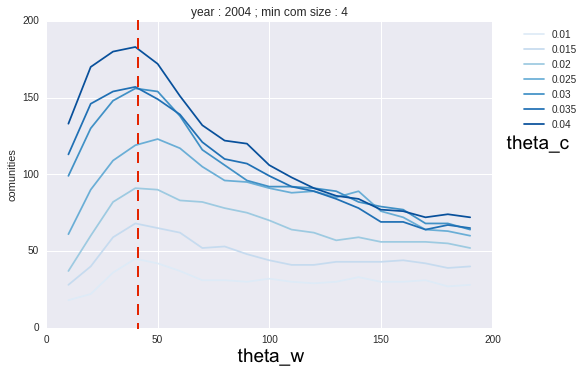
\includegraphics[width=0.55\textwidth,height=0.25\textheight]{figures/comsizes_refined_EDITED}
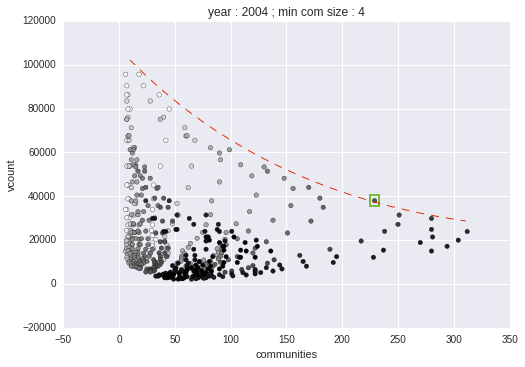
\includegraphics[width=0.55\textwidth,height=0.25\textheight]{figures/pareto_comnum-vcount_color-mod_EDITED}
% TODO redo figures
\caption{\textbf{Sensitivity analysis of network community structure to filtering parameters} We show plot for one example year (2000-2004), all years having the same qualitative behavior (see Supp. Material \ref{XX}) \textit{(Left)} Number of communities as a function of $\theta_w$ for different $\theta_c$ values. The maximum is roughly stable across $\theta_c$ (dashed red line) and years when normalized by patent number, yielding the choice of $\theta_w^{(0)} = 4.5\cdot 10^{-5}$. \textit{(Right)} To choose $\theta_c$, we do a Pareto optimization on communities and network size: the compromise point (green overline) on the Pareto front (red dashed line; grey level gives modularity) gives $\theta_c = 0.06$.\comment{Comment pour la Figure 1: Yo: $\theta_w$ et $\theta_c$ devrait etre ecrit comme dans latex, et dans le meme format que le reste des axes/legende je pense. communities est un nombre positif, donc il faut enlever la partie jusqua -50 sur la figure de droite. Pareil pour vcount. min com size correspond a quoi ? De meme, vcount n'a pas ete defini pour le moment. Quand tu dis "communities" tu sous-entends "number of communites" ? Aussi, le titre des deux graph est le meme, i.e. year: 2004 ; min com size. Je pense qu'il faut soit le diferencier, soit ne pas le mettre du tout. Finalement, la legende doit etre ultra precise, mais au pire des cas je changerai ca a la fin quand tu auras repondu a toutes ces questions :) a-t-on vraiment besoin de preciser que les autres annees sont similaires dans la legende de la Figure? Le reviewer se doute bien que tu ne vas pas plotter les 30 annees. Je pense que c'est mieux de mettre ca dans le corps du texte. Desole pour tous ces retours techniques, mais je me suis fait tellement deboite dans mes DM en PhD :p}}
\label{fig:networksensitivity}
\end{figure}
%%%%%%%%%%%%%%%%%%%%%%

%%%%%%%%%%%%%%%%%%%%%%
\begin{figure}
\centering
\hspace*{-7cm}
\includegraphics[width=0.75\textwidth]{figures/graph-filtered_2000-2004_kwLimit100000_dispth0_06_ethunit4_5e-05_LOWRES}
\caption{\textbf{An example of semantic network visualization.} We show the network obtained for the window 2000-2004, with parameters $\theta_c = 0.06$ and $\theta_w = \theta_w^{(0)}\cdot N_P = 4.5e^{-5} \cdot 9.1e^{5}$. The corresponding file in a vector format (\texttt{.svg}), that can be zoomed and explored, is available as Supplementary Material.}
\label{fig:rawnetwork}
\end{figure}
%%%%%%%%%%%%%%%%%%%%%%


%%%%%%%%%%%%%%%%%%%%%%
\subsection{Characteristics of Semantic Classes}

% content, number of classes in time
% description

% find an example of a patent which was really innovative and for which semantic classes give an insight


Both technological and semantic classes exhibit a hierarchical structure in the sense of a power-law type of distribution of class sizes, as shown in Fig.~\ref{fig:class-sizes}.



\textit{Describe structure of classes (cf graphs hierarchy) ; examples ; Anto case study here ?}

[TBD: ANTO (ETA: 2 days)]




%%%%%%%%%%%%%%%%%%%%%%
\begin{figure}
\centering
\hspace*{-2.5cm}
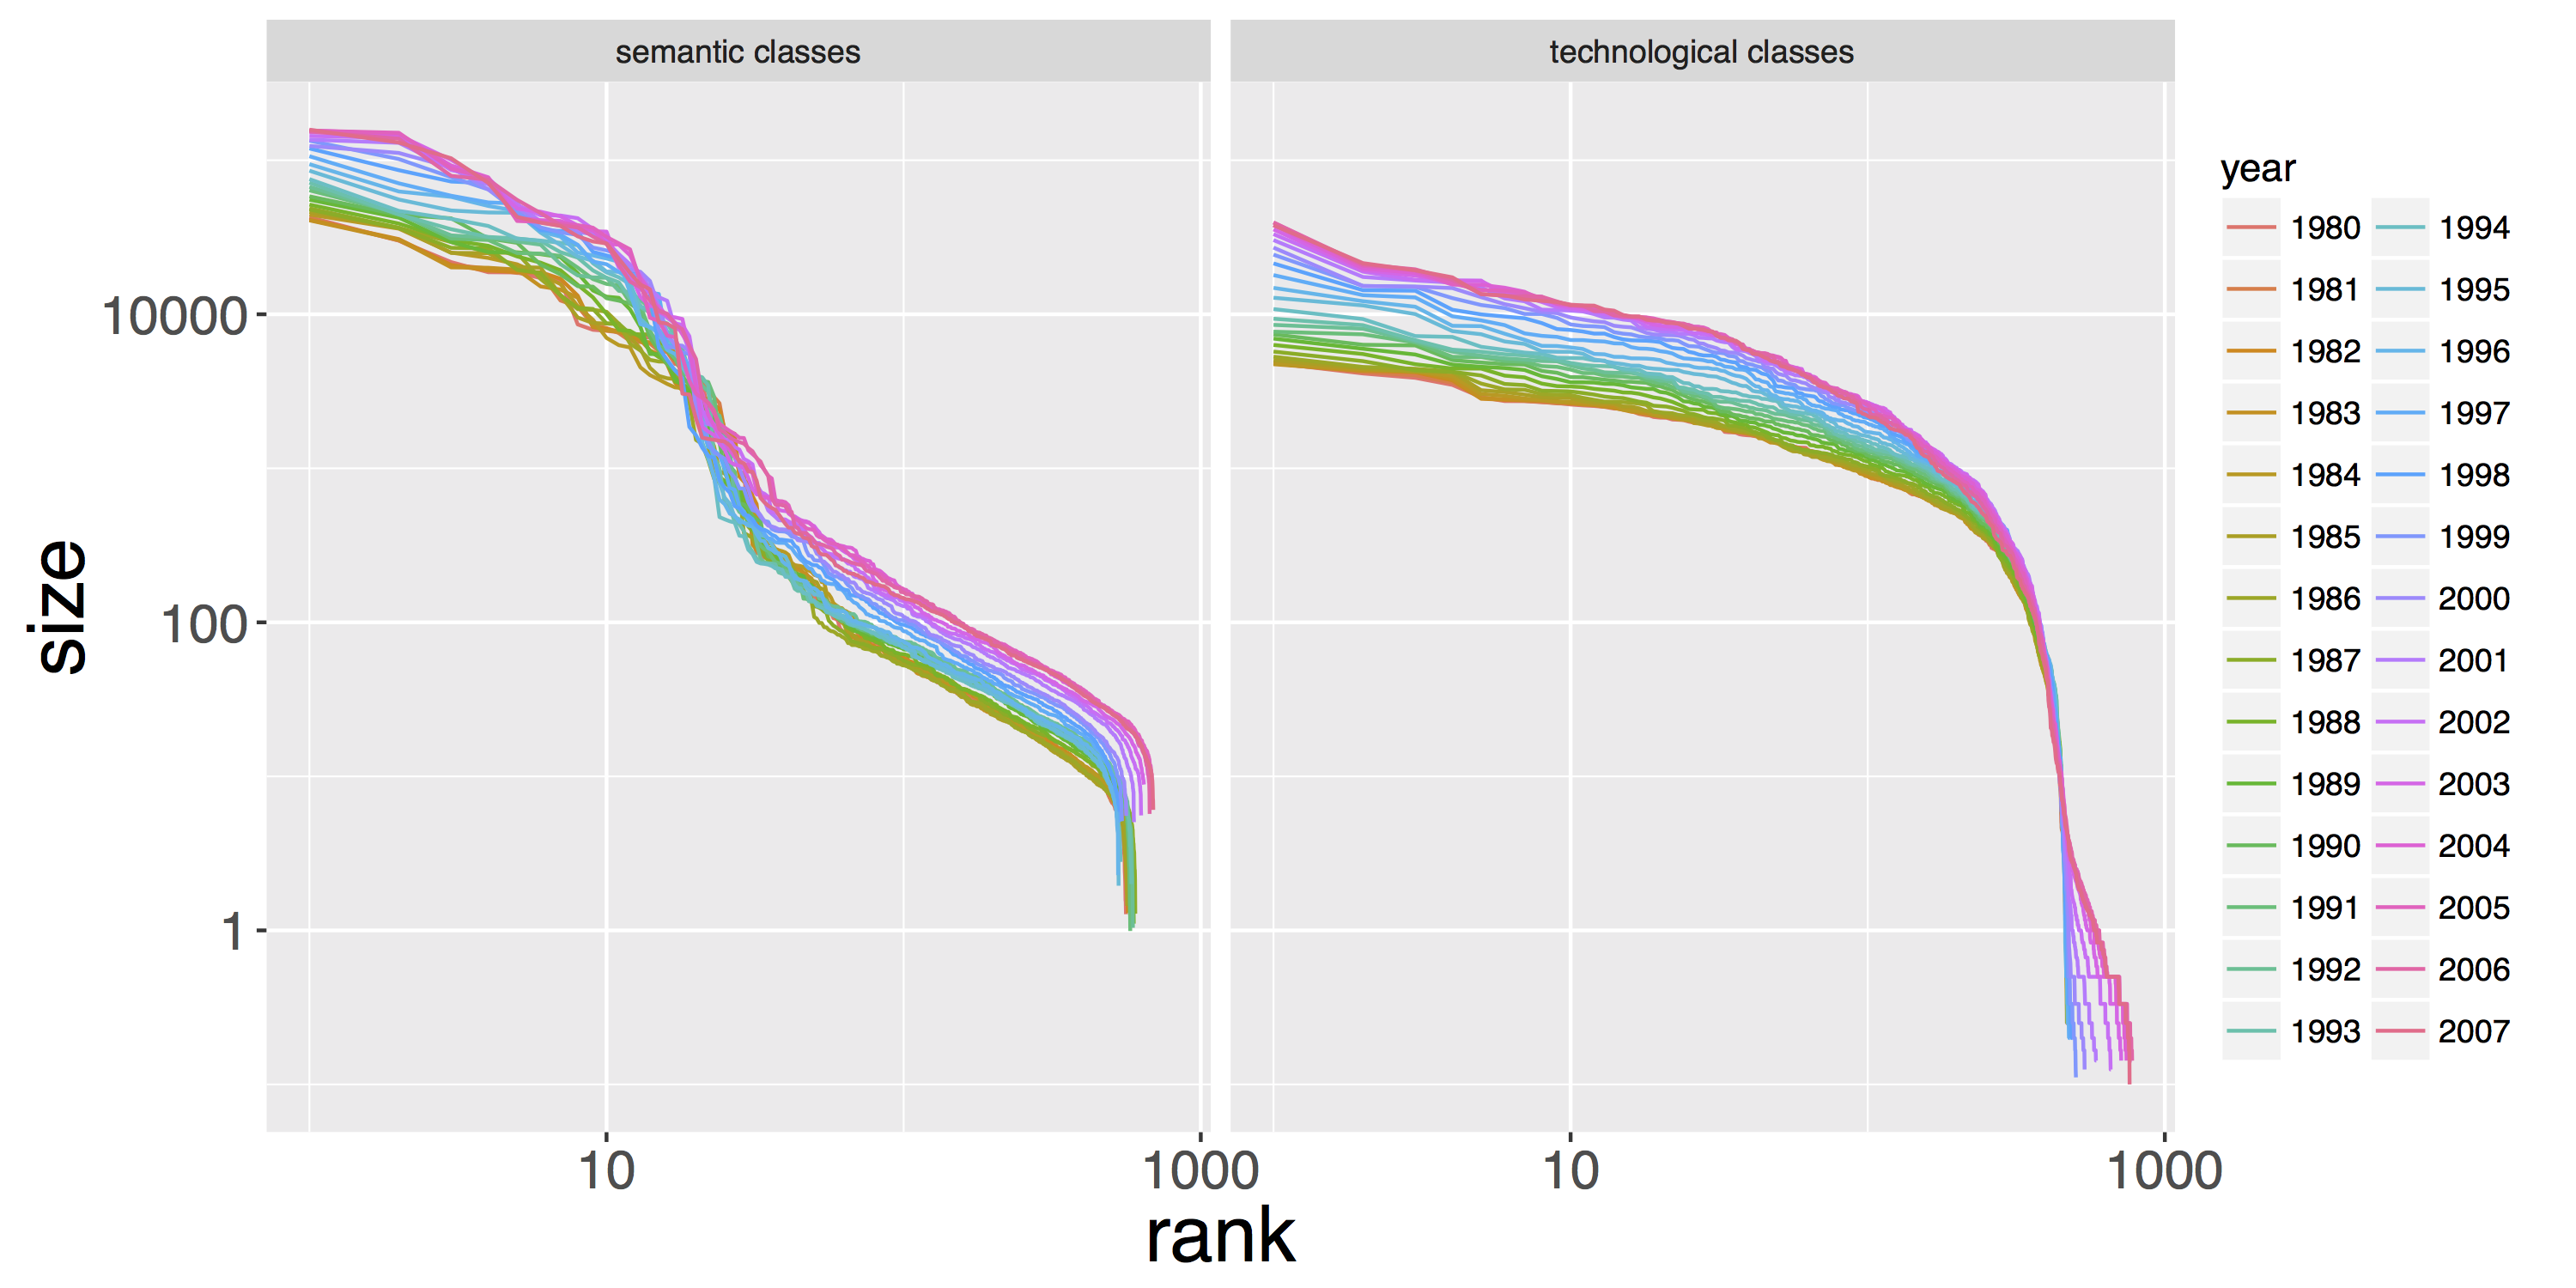
\includegraphics[width=1.2\textwidth]{figures/all_raw_counts}
\caption{Yearly from 1960 to 2012, we plot the log-sizes when restricting to patents which appeared during the corresponding year of semantic classes (left-side) and technological classes (right-side) as a function of their log-rank from the biggest to the smallest. Sizes are computed as the sum over patents of probabilities to belong to the class. Each color corresponds to one specific year. Yearly semantic classes and technological classes present a similar hierarchical structure which confirms the comparability of the two classifications. This feature is crucial for the statistical analysis in Section \ref{statisticalmodel}. Over time, curves are translated and levels of hierarchy stays roughly constant. \comment{(Juste) du coup pour cette figure j'ai laissé les échelles telle quelles pour comparabilité entre les deux ; j'ai précisé que size = sum(probas) ; peut être qu'il faudrait bouger la def des probas pour à la fois sémantic et techno en section 3.4. Sinon pour titres/légendes/axes ça vous va ?}
}
\label{fig:class-sizes}
\end{figure}
%%%%%%%%%%%%%%%%%%%%%%






%%%%%%%%%%%%%%%%%%%%%%
\section{Results \label{result}}
%%%%%%%%%%%%%%%%%%%%%





%%%%%%%%%%%%%%%%%%%%%%
\subsection{Semantic Communities Dynamics \label{subsec:semantic-flows}}

% this section describes semantic communities reconstruction and their temporal dynamics

A first insight into innovation dynamics can be drawn from the analysis of semantic communities dynamics. Communities are constructed yearly and thus one can define proximity between two successive communities $S_i(t)$ and $S_j(t+1)$ using a set similarity index between both sets of keywords, defined as the normalized intersection $j(A,B)=2\cdot \frac{\left|A\cap B\right|}{\left|A\right|+\left|B\right|}$, where $\left|X\right|$ corresponds to the cardinal of $X$. It enables us to infer flows of topics between communities in time and answer specific questions such as the potential precursors of one specific innovative fields. We show in figure~\ref{fig:semanticflows} a sample of these flows for the largest classes.
\comment{En dire un peu plus sur la convergence des technologies. Est ce qu'on observe bien la convergence là dedans?}


\todo{Expected results : succession of classes in time ; maybe "unexpected flows" : ex how \texttt{hydrogen} divides ; birth of classes and dynamics reveal the evolution of technology in time. Seems to have some fusions/birth in the preliminary graph ; first need to have a clean graph to then look at some particular aspects.}



%%%%%%%%%%%%%%%%%%%%%%
\begin{figure}
\centering
% full flow graph or a snapshot depending on readability on all years and all classes

%  Sankey network of Citation flows ? -> not relevant to my mind

\hspace*{-2.5cm}
% placeholder figure for now
%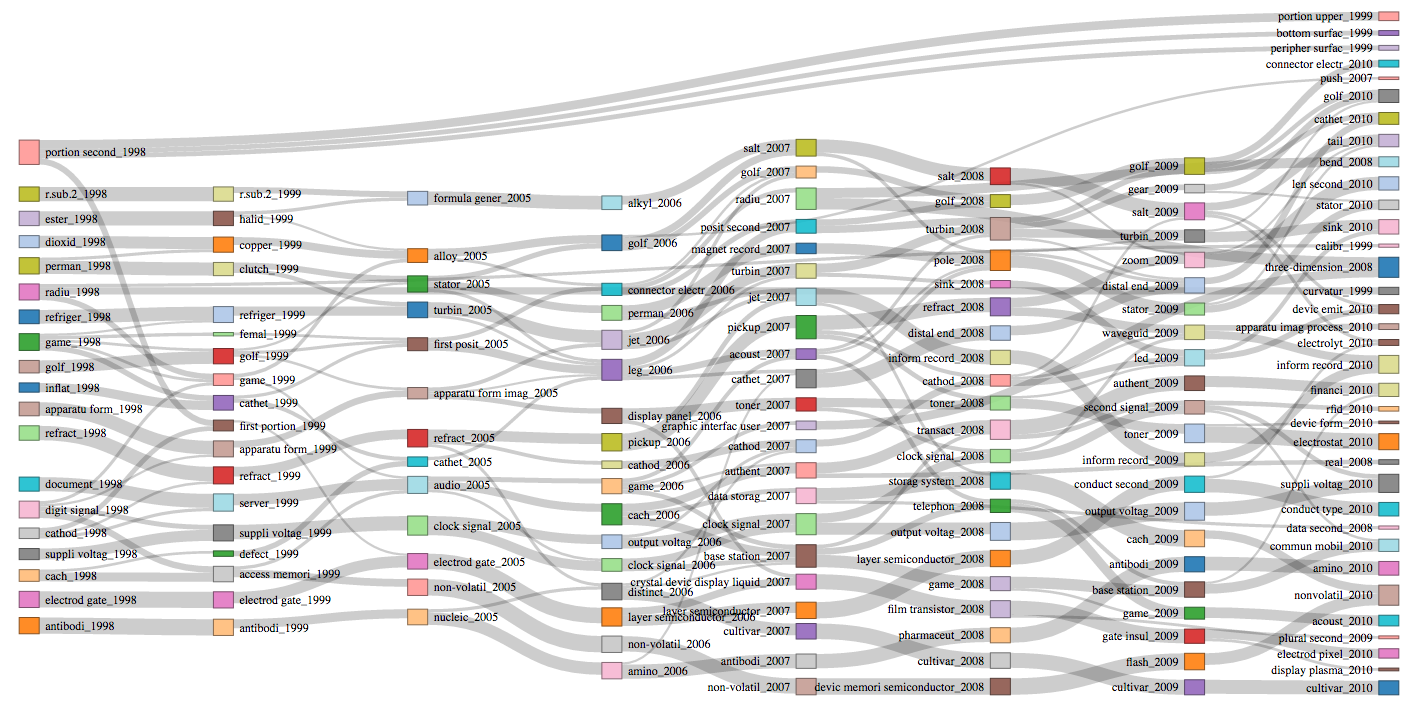
\includegraphics[width=\textwidth]{figures/example_semanticFlows_1998-2010}
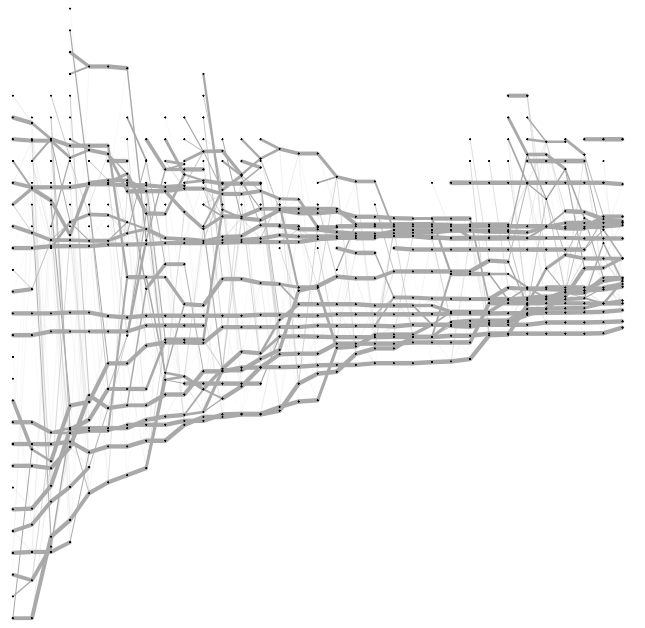
\includegraphics[width=1.2\textwidth,height=0.4\textheight]{figures/test_flows_layoutProximity}
\caption{\textbf{Semantic flows between successive classes in time.} We take each year the 3\% larger classes. \comment{(Juste) Cette figure est horrible et provisoire ; je dois creer of scratch un algo de layout parce que le package que j'utilisais est moisi, c'est super galère, pour l'instant c'est un greedy mais du coup il a un biais structurel que les branches tendent à converger ; je vais essayer une optim sur l'ensemble des angles pour minimiser l'angle total des branche pondérés ; pour les noms je ferai apparaitre ceux des plus grosses classes seulement}[Question sur les noms, on est obligé de mettre les stem ce que je comprends mais du coup c'est pas toujours évident de comprendre... On peut faire un link stem $\rightarrow$ most used kw ?]\comment{arf chaud là comme ça, je l'ai pas memorisé lors de l'extraction des stem parce que je voulais pas prendre trop de memoire, il faudrait coder ça et refaire tourner.. (j'ai toujours pas accès au serveur :/ )}}
\label{fig:semanticflows}
\end{figure}
%%%%%%%%%%%%%%%%%%%%%%



%%%%%%%%%%%%%%%%%%%%%%
\subsection{Patent Level Diversity}

Given a classification system (technological or semantic classes), given by probabilities $p_{ij}$ for each patent $i$ to belong to class $j$ \comment{Yo: C'est la premiere fois qu'on definit $p_{ij}$, je pense qu'il est necessaire d'etre un peu plus clair sur ce que c'est. L'explication qu'on donne dans le paragraphe d'apres est encore plus floue en premiere lecture. Je comprends le truc car je suis coauteur, mais je ne pense pas qu'un reviewer comprendrait en premiere lecture. (Anto) Oui je suis d'accord, il faudrait expliquer que conceptuellement c'est différent des classes techno car on a des proba d'appartenance, et même dans les classes techno, ce n'est pas trivial que la proba d'appartenir à chaque classe est égal à 1/N, c'est une hypothèse que l'on fait}[(Juste) est ce que ça vous semblerait pertinent de bouger la def des probas à la fois pour sémantique et techno en 3.4, parce qu'on les utilise déjà pour les tailles en fait, et plus tôt c'est le mieux car le concept est central par la suite], one can define a patent-level diversity measure as one minus the herfindhal index \comment{c'est classique le herfindhal ?} on $p_{ij}$ by:

\[
D_i = 1 - \sum_j {p_{ij}^2}.
\]

For the semantic classification, these probabilities are computed over classified keywords of a patent: taking all potential keywords yield very small probabilities (as a lot of keywords are not nodes of the semantic network) and may include bias due e.g. to the variation of abstract length in time. For technological class, there is no probability directly associated with each class. We considered for this reason that each class received a probability equal to 1 over the total number of patent $i$'s technological classes, generalizing the technological classification in a way comparable to the semantic classification. \comment{Yo: C'est pas mal quand meme l'explication, mais il faut vraiment qu'on betonne ca en reformulant quelques trucs :) Par exemple, le biais est plus embrouillant qu'autre chose en premiere lecture. Il devrait venir apres les definitions claires des objets.}

\comment{Yo: IMPORTANT: C'est quoi la definition de $p_{ij}$ pour les classes technologiques (je ne comprends pas la derniere phrase en fait)}[c'est écrit au dessus ``For technological class,... comparable to the semantic classification'' ; il faudrait peut etre le reformuler. les probas technos des patents, c'est 0 s'il apprtient pas à la classe, 1/son nombre de classes s'il y appartient]\comment{ok, j'avais loupe quelque chose, c'est de ma faute. Je vais essayer de re-ecrire un poil cette partie!}

\comment{Je pense qu'il faut dire un mot sur la définition usuelle de l'originality ou de la generality en classe techno: c'est la même efinition mais en definissant $p_{ij}$ comme la part dans la classe $j$ des brevets citants ou étant cités par le brevet $i$ dans les 5 ans. Je vais le calculer pour les classes semantiques.}[très bonne idée, du coup on peut splitter cette partie en diversity et originality/generality ; ça donne un équivalent de 4.4 et 4.5 mais au niveau du patent]
We show in Figure~\ref{fig:patent-level-orig} the distribution over time of semantic and technological diversity with the corresponding mean time-series. This is carried with two different settings, namely including/not including patents with zero diversity (single class patents). We call other patents ``complicated patents'' in the following. First of all, the presence of mass in small probabilities for semantic but not technological diversity confirms that the semantic classification contains patent spread over a larger number of classes. More interestingly, a general decrease of diversity for complicated patents, both for semantic and technological classification system, can be interpreted as an increase in invention specialization. This is a well-known stylized fact as documented in~\cite{ARCHIBUGI199279}. Furthermore, a qualitative regime shift on semantic classification occurs around 1996. This can be seen whether or not we include patents with zero diversity. The diversity of complicated patents stabilizes after a constant decrease, and the overall diversity begins to strongly decrease. This means that on the one hand the number of single class patents begins to increase and on the other hand complicated patents do not change in diversity. It can be interpreted as a change in the regime of specialization, the new regime being caused by more single-class patents. This effect does not seem to be spurious neither with patent count nor with network size. \textcolor{red}{do we add the corresponding figures as supplementary to justify this ?}\textcolor{blue}{Yo: soit on l'ajoute as supplementary material en referencant, soit on enleve la phrase}


%\textit{Row 2 of the corresponding figure Fig.\ref{fig:patent-level-orig} will be kept ; we evoke row 1 saying that keywords are more difficult to classify in time (increase of diversity $\iff$ smaller probas $\iff$ ``biais'' due to longer abtrsacts, more complicated inventions etc.  )} % TODO plot length of abstracts in time. Rq : we could have taken a total number of kws linked to mean abstact length.. but a level of complication more..
%\textit{thus we work with probas computed on \textbf{classified keywords}. Try to interpret the peak in semantic; it is not a direct bias due to patent count, as begins to decrease in 96; when removing zero-originality patents (third row), clear decreasing trend for semantic as for techno : interpretation : apparent increase of diversity was due to a decrease of single class patent ; but considering only multi-class patents semantic follows techno. Can it have an economic interpretation ?}


%%%%%%%%%%%%%%%%%%%%%%
\begin{figure}

%First row : semantic with all keywords ; 
%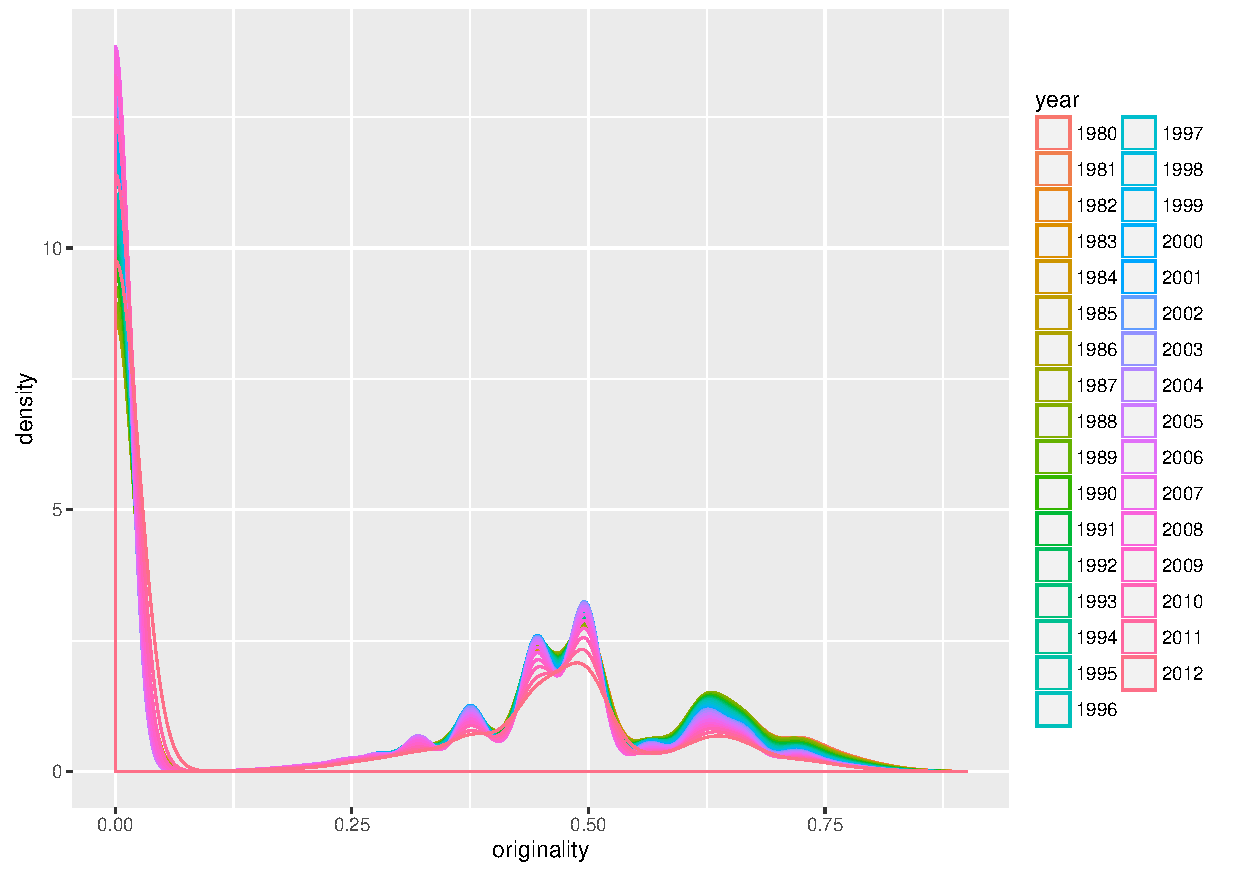
\includegraphics[width=0.24\textwidth,height=0.15\textheight]{figures/patentlevel-origs-techno}
%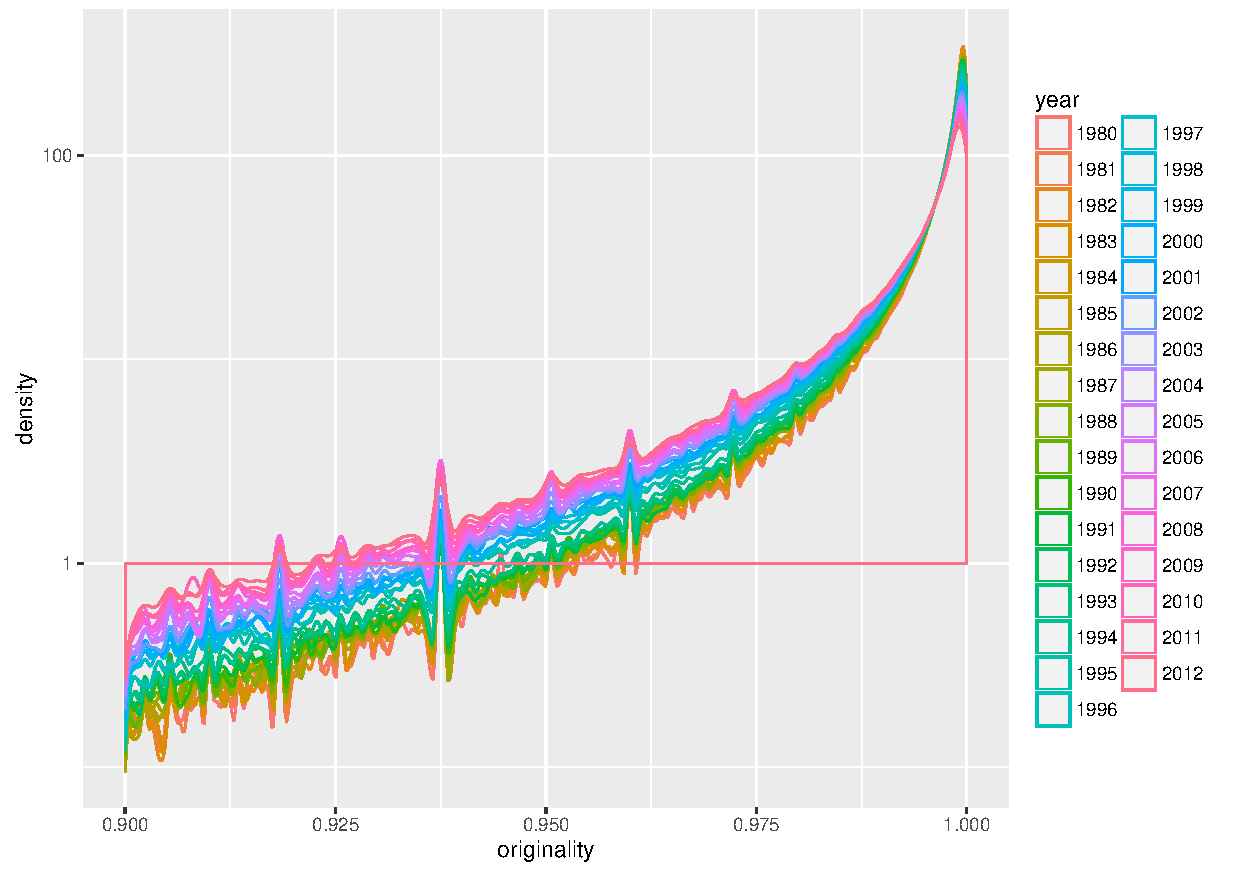
\includegraphics[width=0.24\textwidth,height=0.15\textheight]{figures/patentlevel_semorigs_high_logscale}
%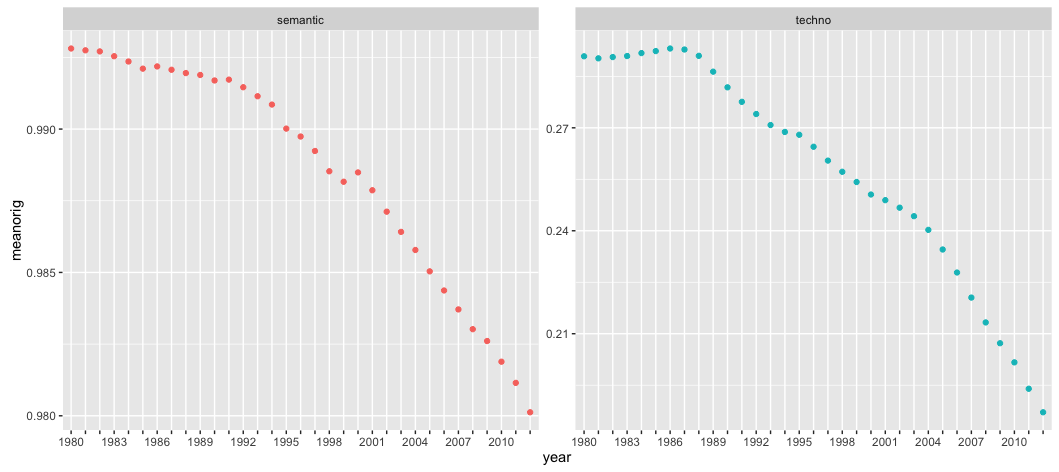
\includegraphics[width=0.45\textwidth]{figures/patentlevel-origs-mean-ts}
%\\
%First row : semantic with relevant keywords only - all patents 
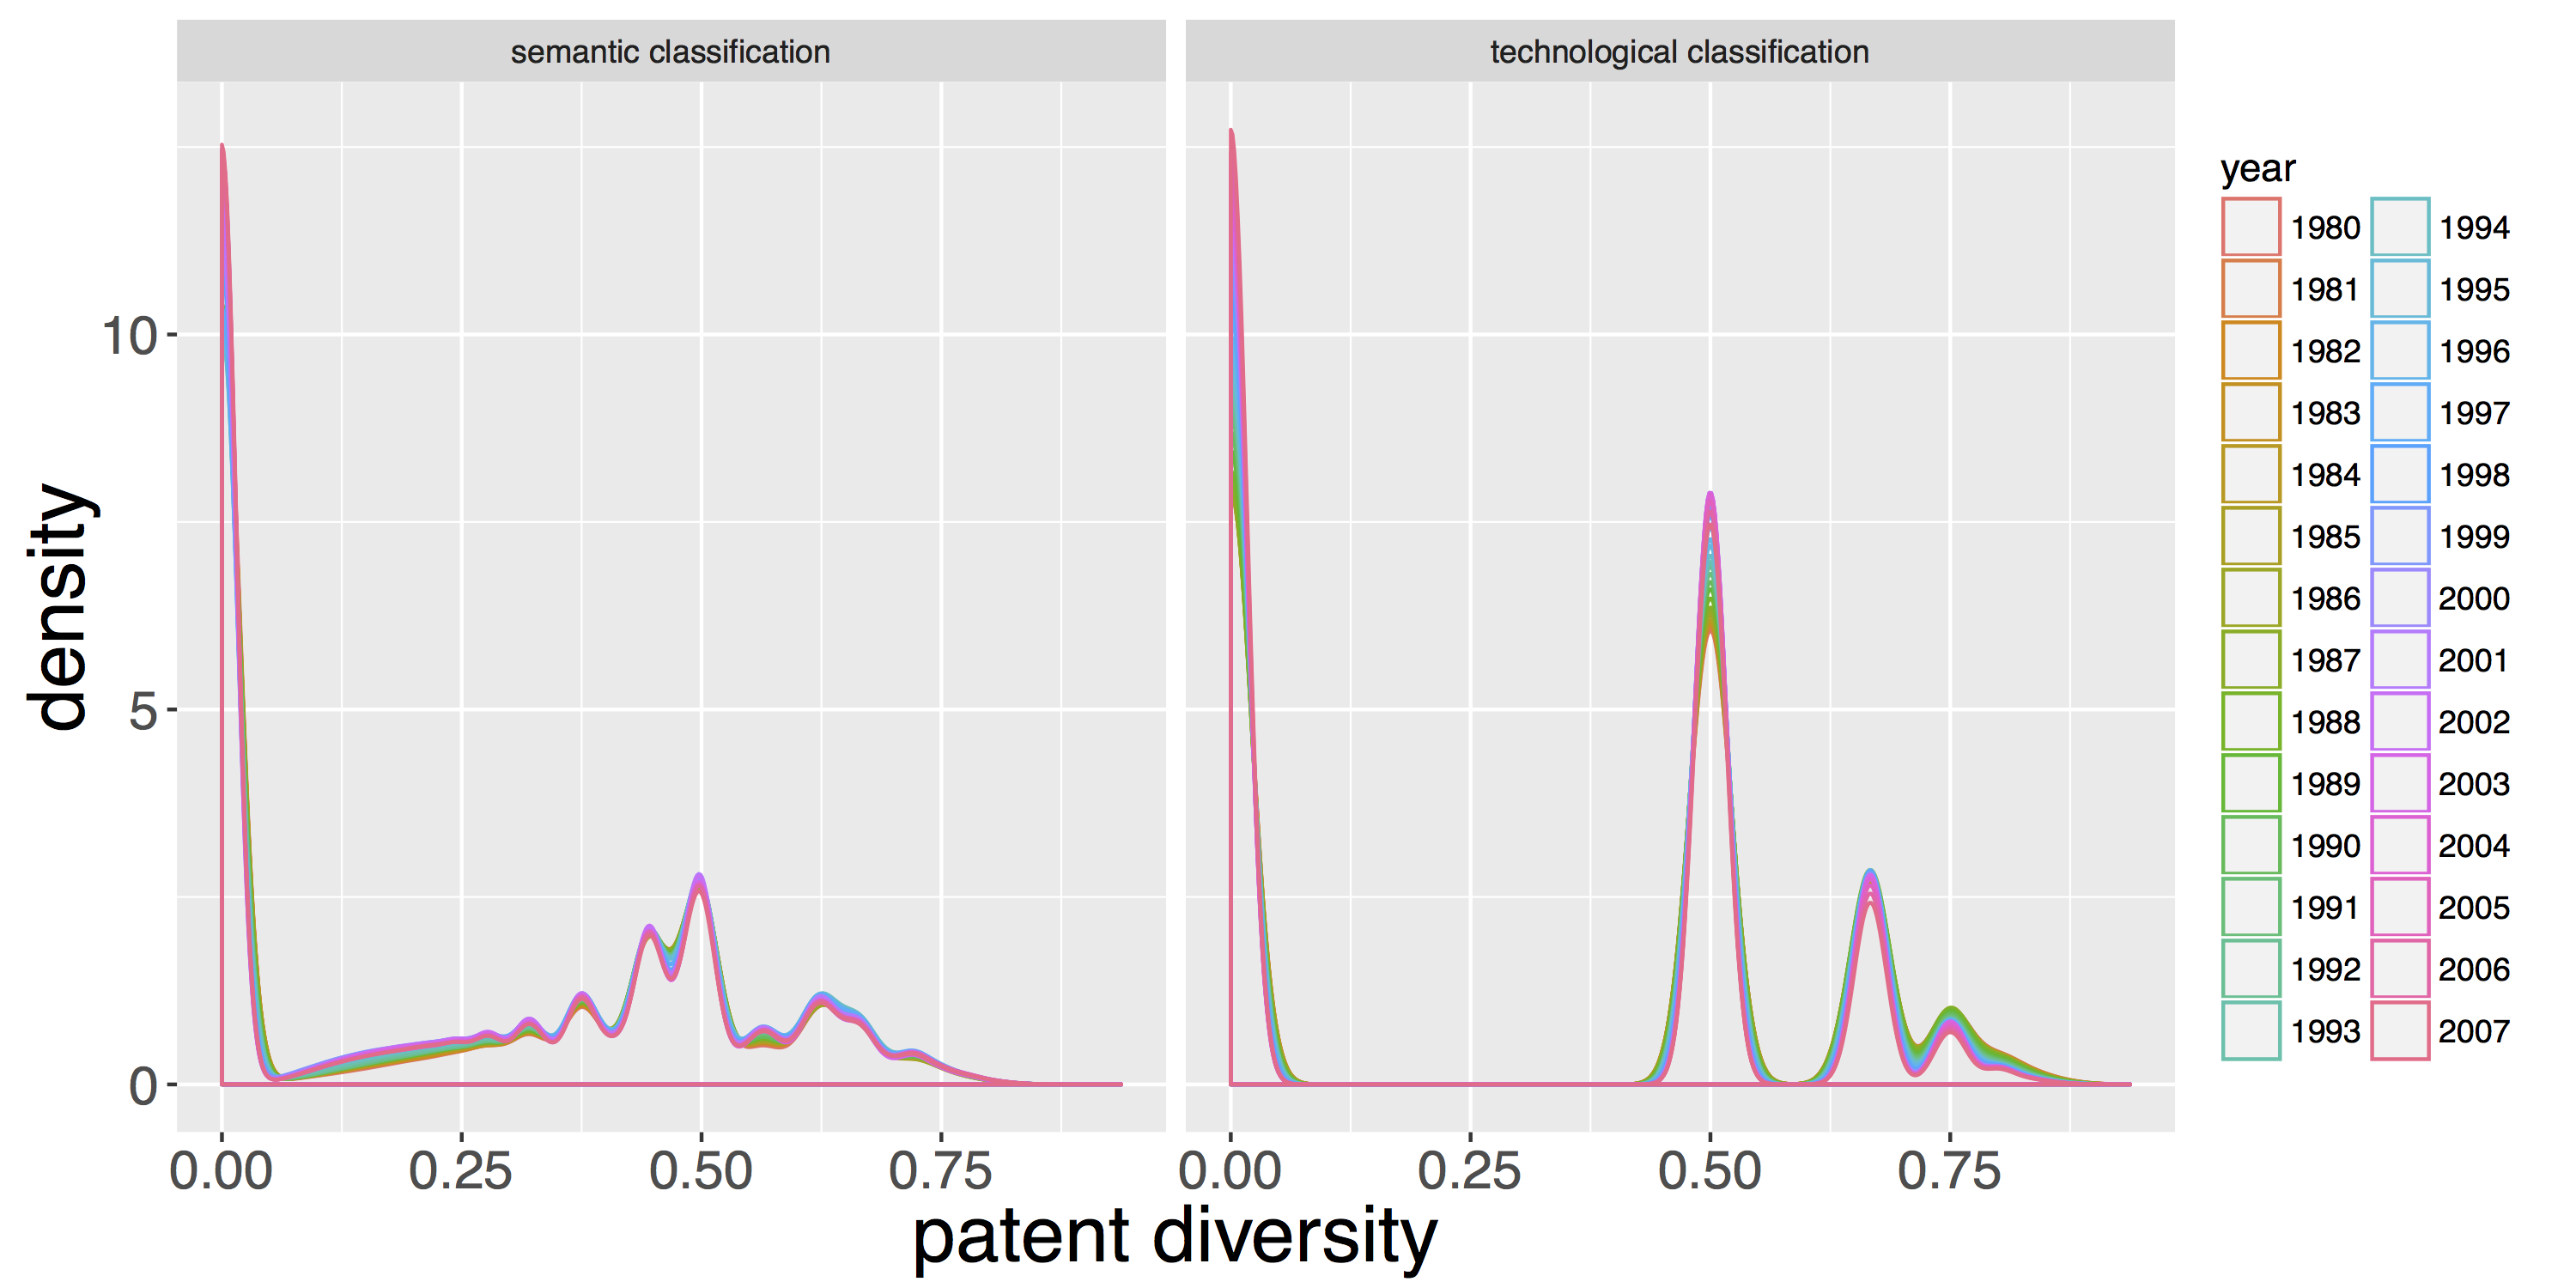
\includegraphics[width=0.49\textwidth]{figures/patentlevelorigs_all_semcounts}
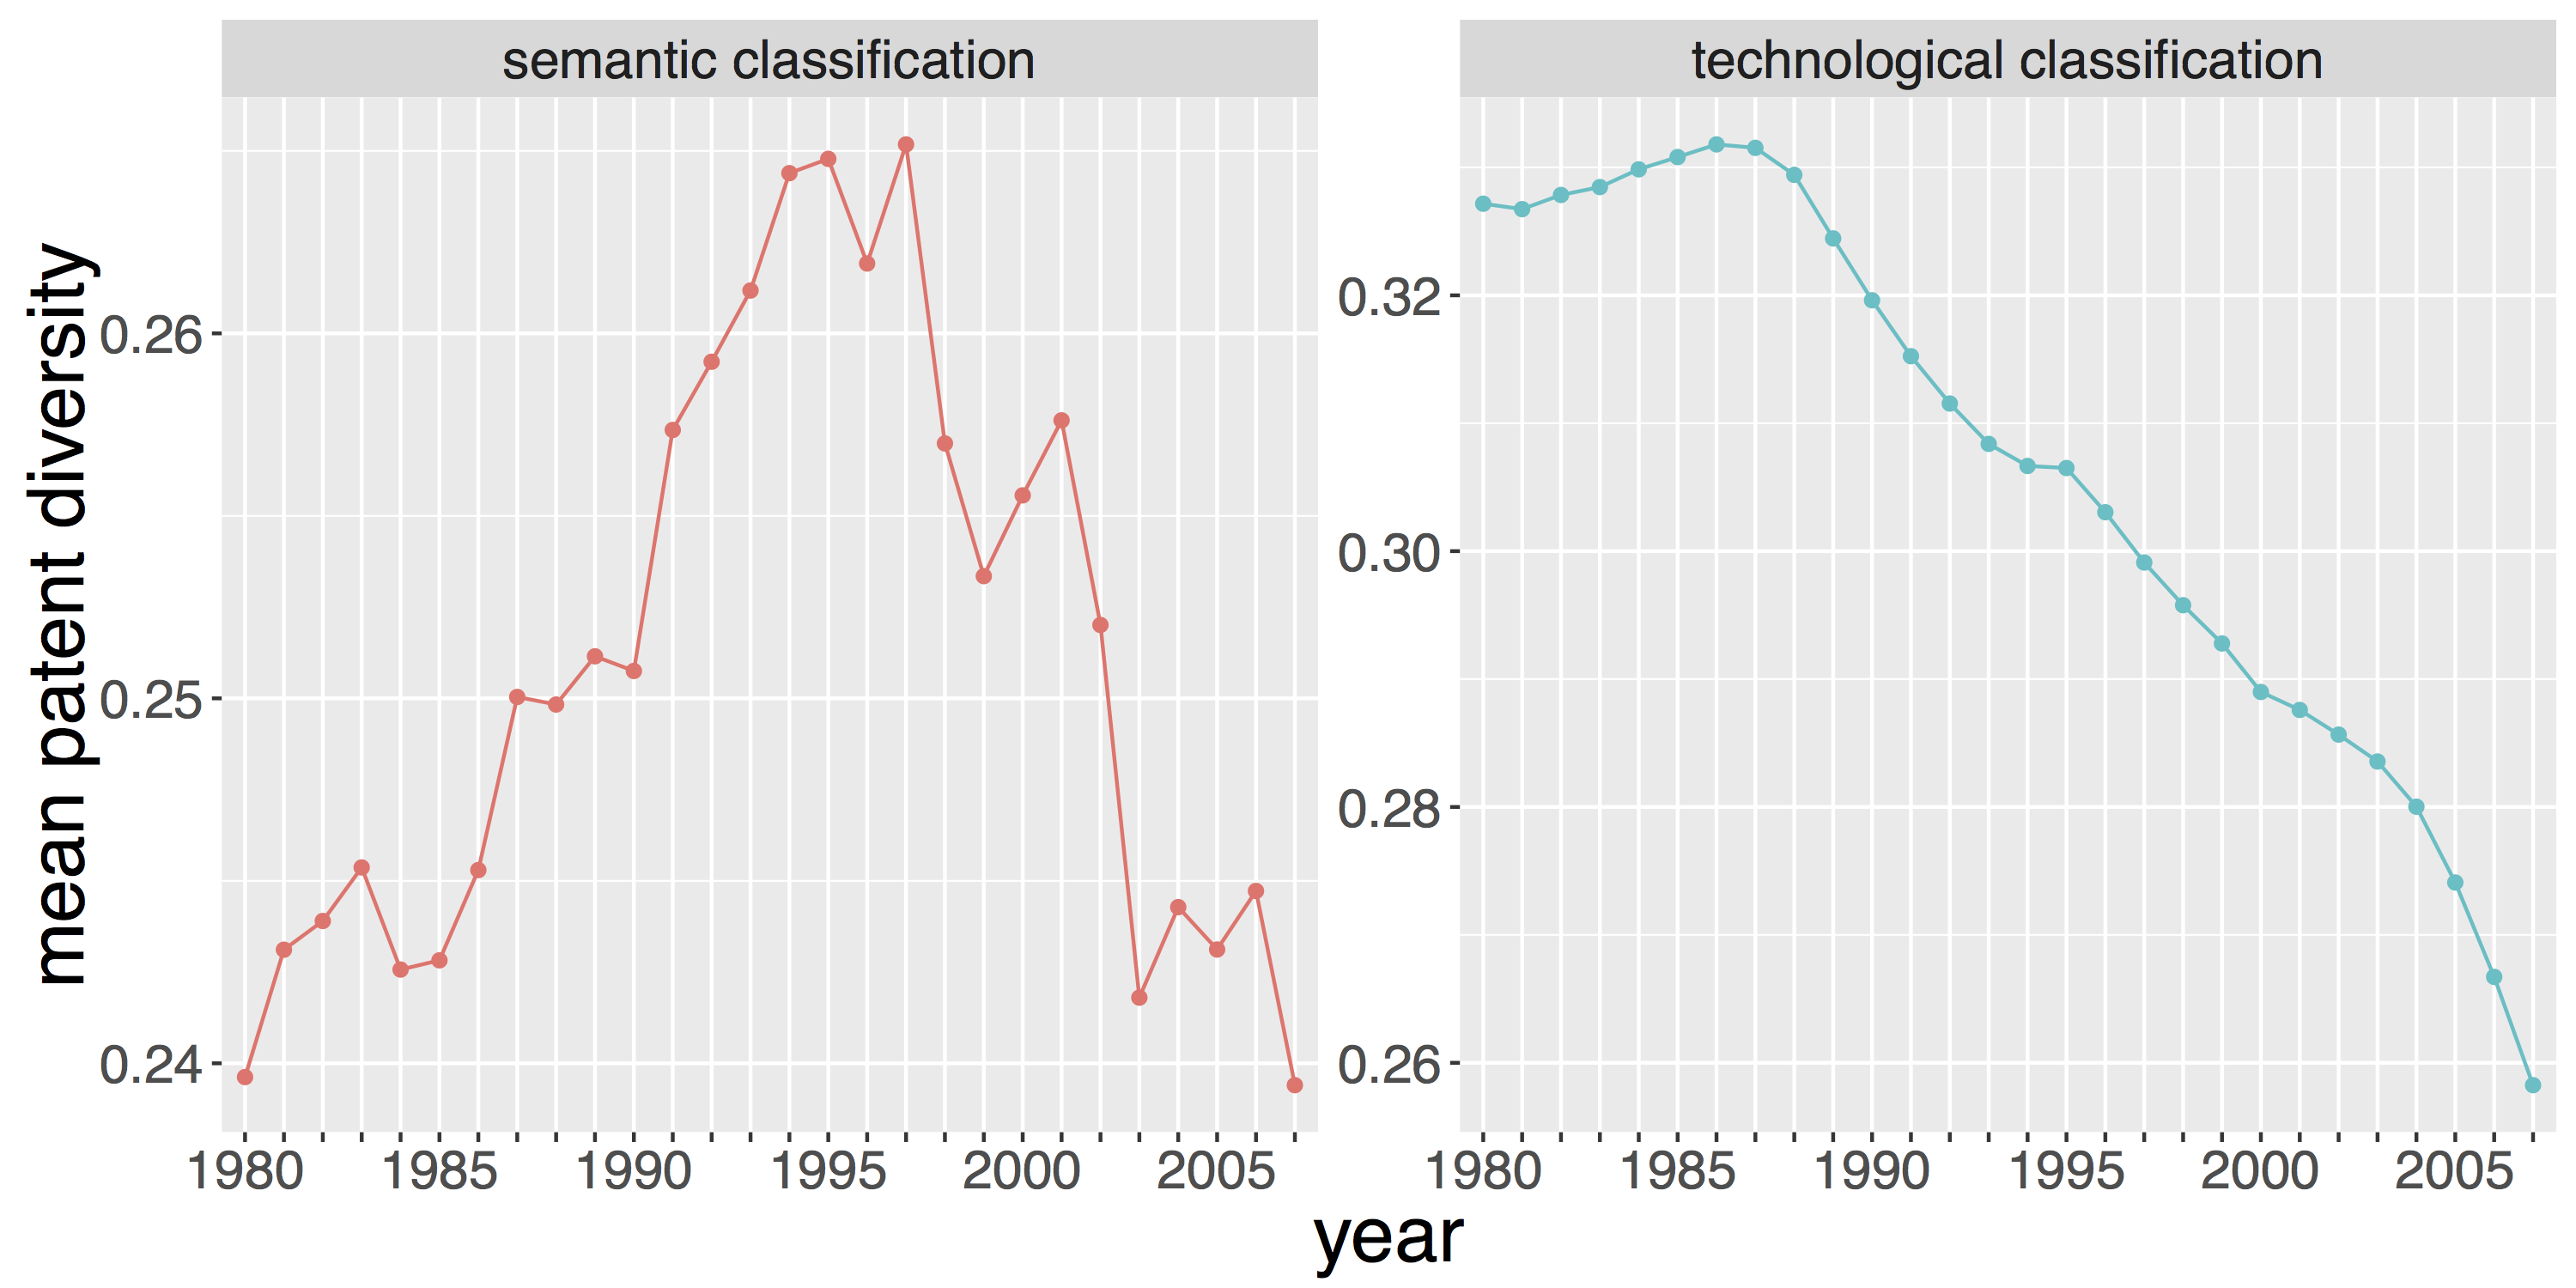
\includegraphics[width=0.49\textwidth]{figures/patentlevelorigs_all_ts_semcounts}\\
%Second row : patents with diversity $> 0$ (more than one class)}
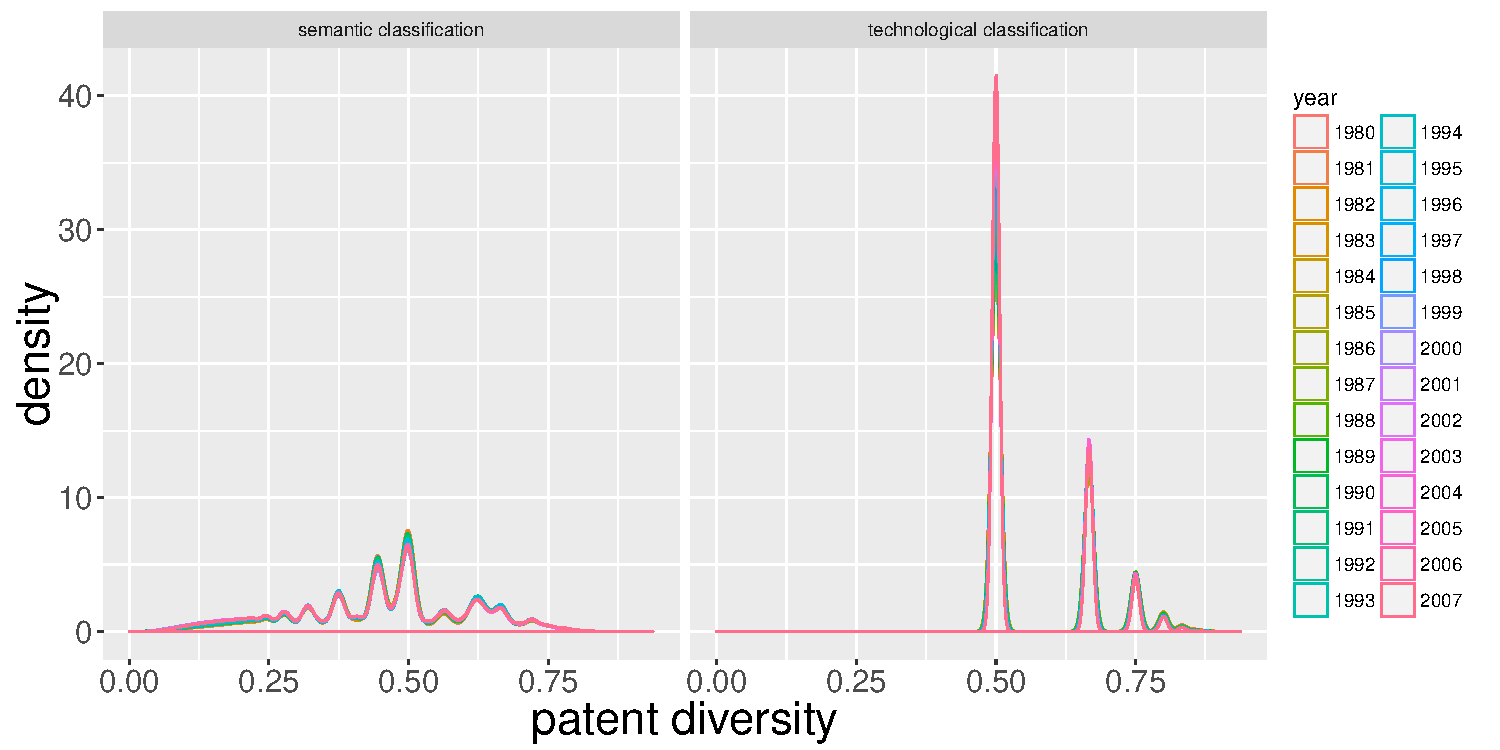
\includegraphics[width=0.49\textwidth]{figures/patentlevelorigs_positive_semcounts}
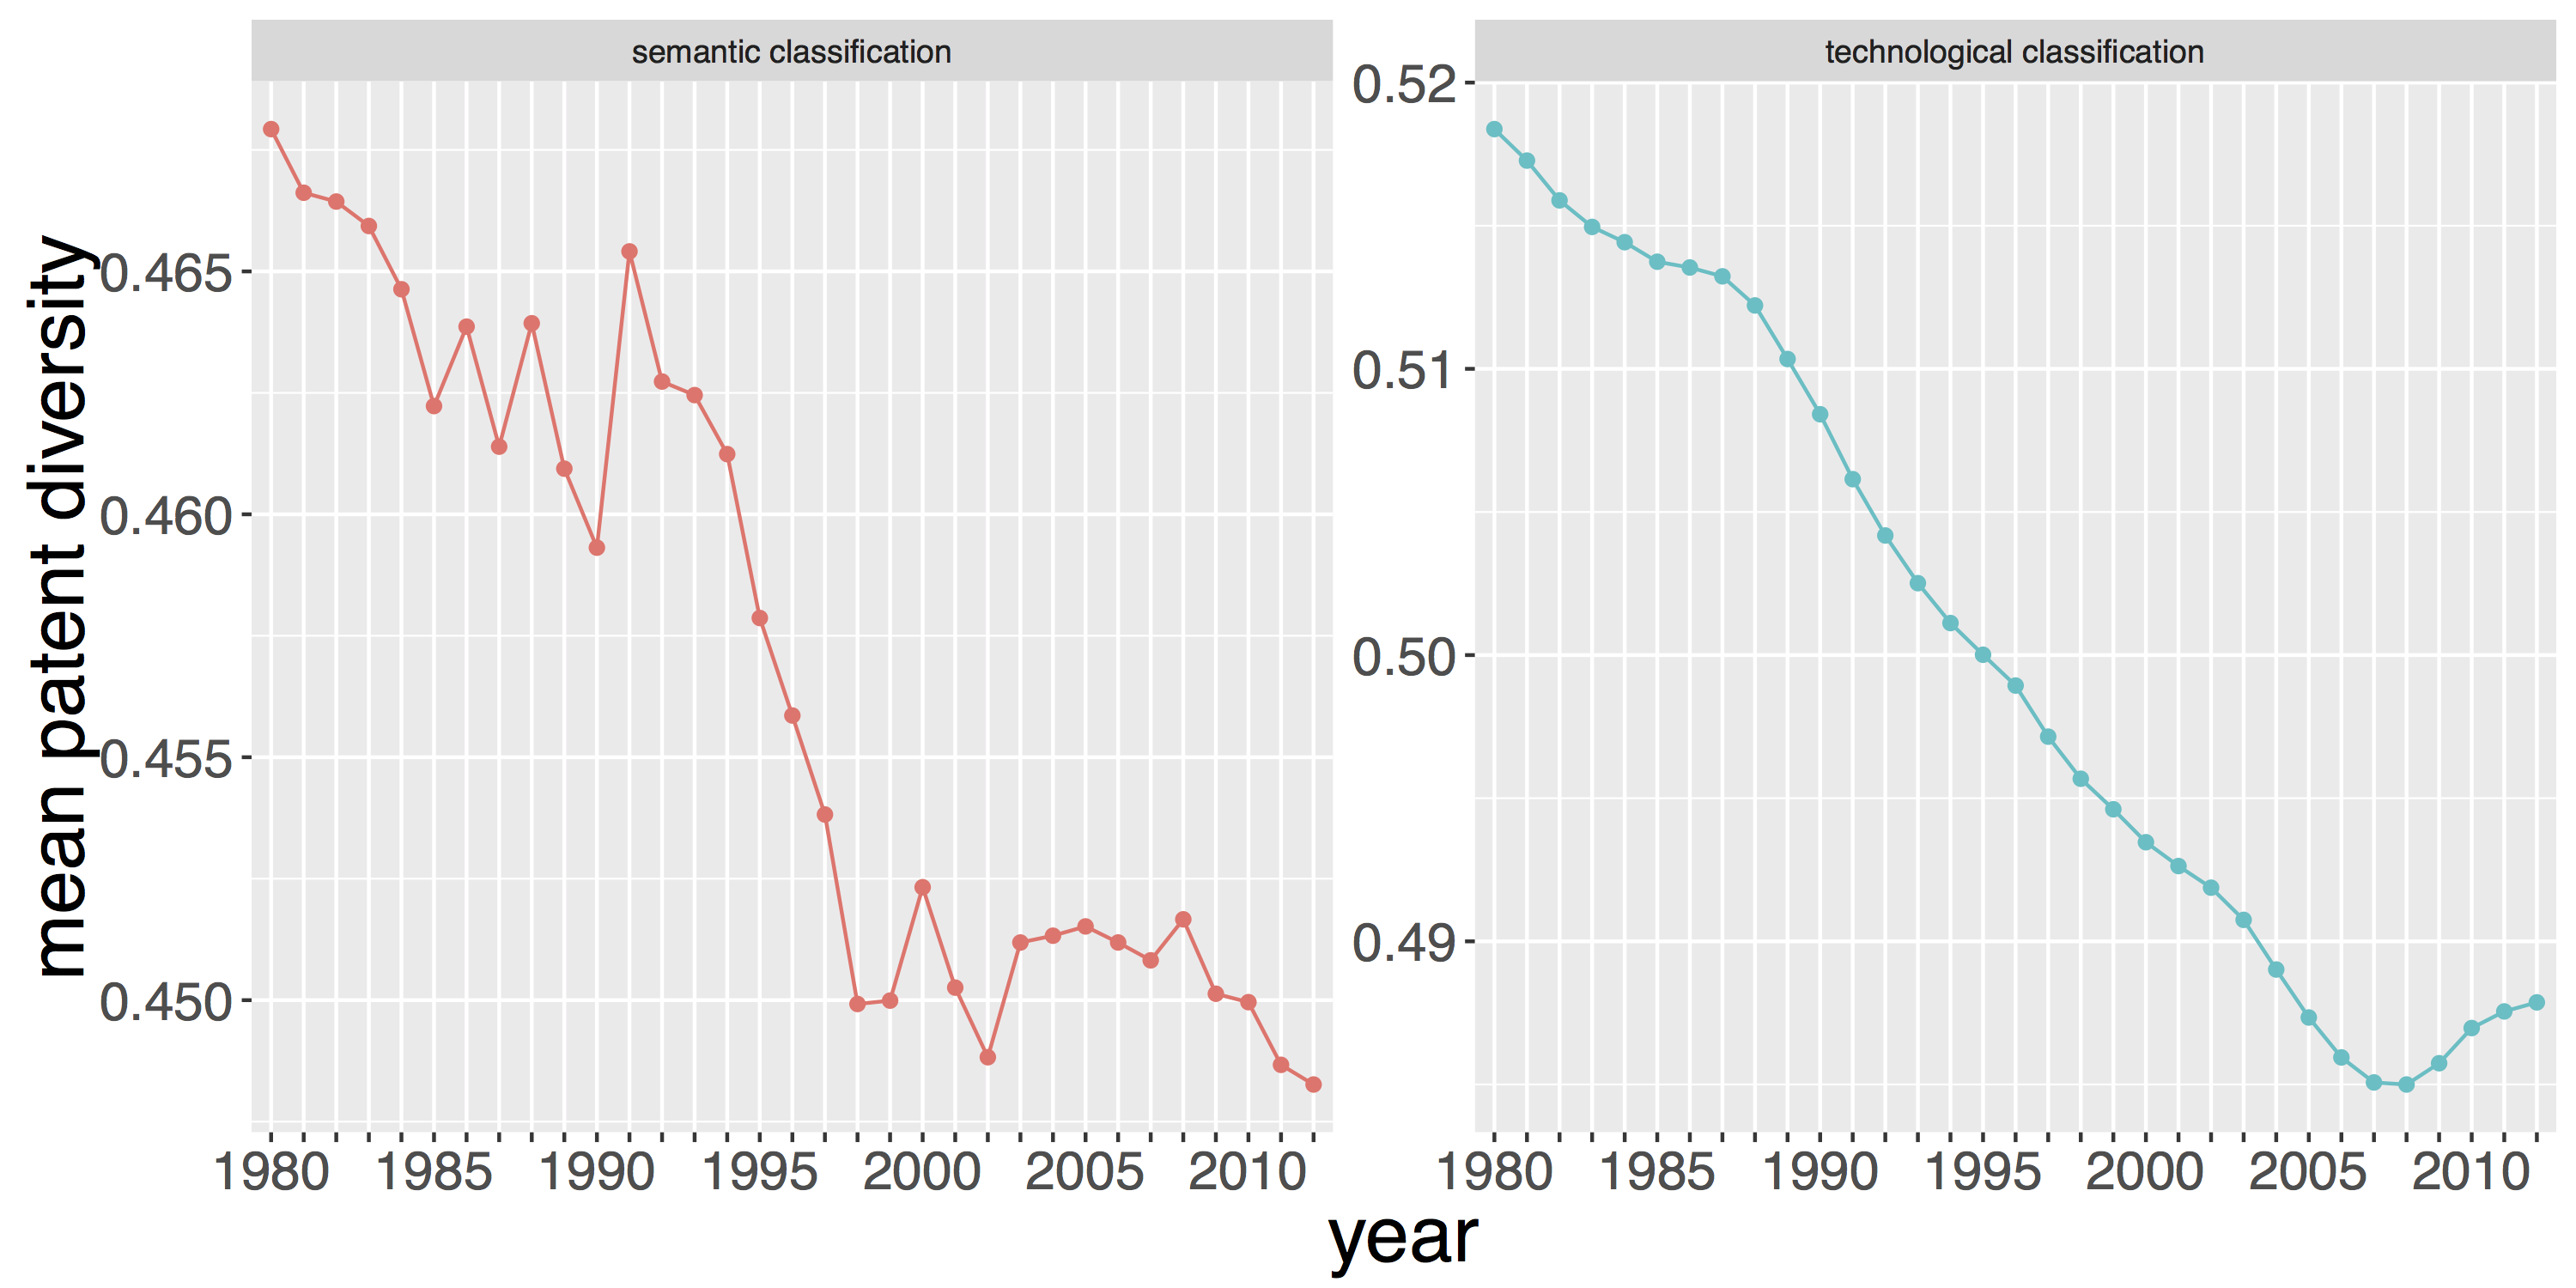
\includegraphics[width=0.49\textwidth]{figures/patentlevelorigs_positive_ts_semcounts}
\caption{
\textbf{Patent level diversities.} Distributions of diversities (Left column) and corresponding mean time-series (Right column). First row includes all classified patents, whereas second row includes only patents with more than one class (i.e. patent with diversity greater than 0). \comment{(Juste) Même question pour les axes/labels, ça vous va ?}
}
\label{fig:patent-level-orig}
\end{figure}
%%%%%%%%%%%%%%%%%%%%%%






%%%%%%%%%%%%%%%%%%%%%%
\subsection{Classes overlaps}

% comparison of techno classes / semantic communities - citation done with modularity and stat method further

A proximity measure between two classes can be defined by their overlap in terms of patents. In a generalized form with class belonging probability matrix $\left(p_{ki}\right)$ (giving for patent $k$ probabilities to belong to each class $i$) it writes $O_{ij} = \frac{1}{N_P}\cdot \sum_{k} p_{ki} p_{kj}$. The overlap is normalized by patent count to remove effect size. The corresponding relative overlap (set similarity defined in section~\ref{subsec:semantic-flows}) is computed the same way.


\paragraph{Intra-classification overlaps}

The study of distributions of overlaps inside each classification, i.e. between technological classes and between semantic classes separately, reveals the structural difference between the two classifications methods, suggesting their complementary nature. Their evolution in time can furthermore give insights into trends of specialization. We show in figure~\ref{fig:intra-classif-overlap} distributions and mean time-series of overlaps for the two classifications. Technological classification globally always follow a decreasing trend (years after 2007 being not significant as stationary regime is not yet reached), what corresponds to more and more isolated classes, i.e. specialized inventions, confirming the stylized fact obtained in previous subsection. For semantic classes, the dynamic is somehow more intriguing and supports the story of a qualitative regime shift suggested before. Although globally decreasing as technological overlap, normalized (resp. relative) mean overlap exhibit a peak (clearer for normalized overlap) culminating in 1996 (resp. 1999). Looking at normalized overlaps, classification structure was somewhat stable until 1990, then strongly increased to peak in 1996 to then decrease at a similar pace until today. Technologies began to share more and more until a breakpoint when increasing isolation became the rule again. An evolutionary perspective on technological innovation~\cite{ziman2003technological} could shed light on possible interpretations of this regime shift: as species evolve, the fitness landscape first would have been locally favorable to cross-insemination, until each fitness reaches a threshold above which auto-specialization becomes the optimal path. It is very comparable to the establishment of an ecological niche~\cite{holland2012signals}, the strong interdependency originating here during the mutual insemination resulting in a highly path-dependent final situation. This interpretation is consistent with the dynamics of semantic flows presented in Fig.~\ref{fig:semanticflows}, as the increase period roughly corresponds to a sequence where inter-class flows are stronger.


\todo{it may be interesting to find the most overlapping semantic classes in 1996 ; and look the closest classes in 1980 and in 2004, to try to have a concrete insight on what happened. Anto could you do that ? Also for this part the most important is to try to interpret the dynamics accurately from an economic point of view, i'm not sure my bla-bla is very relevant economically ; and maybe too long, do not hesitate to shorten !} 



%%%%%%%%%%%%%%%%%%%%%%
\begin{figure}[!ht]
\centering
%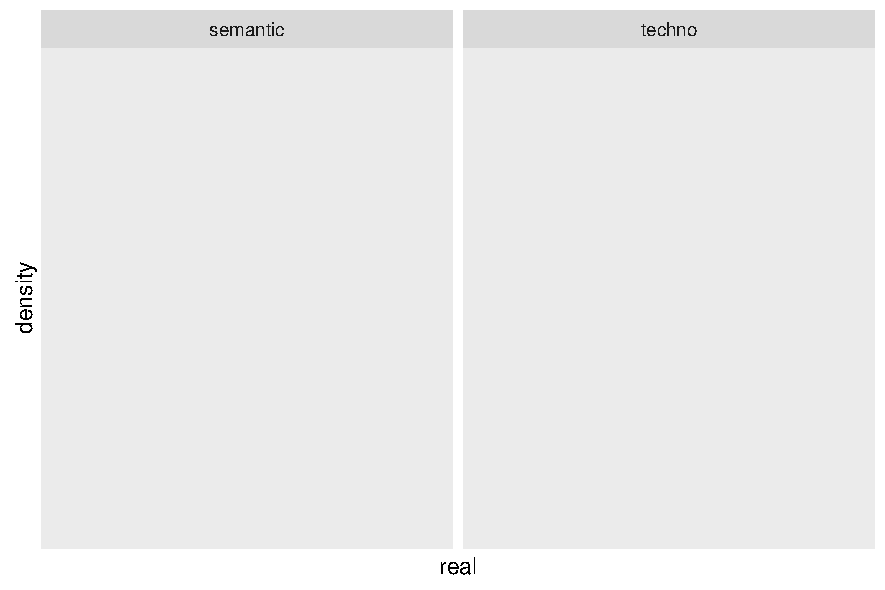
\includegraphics[width=0.49\textwidth]{figures/real_all_density}
%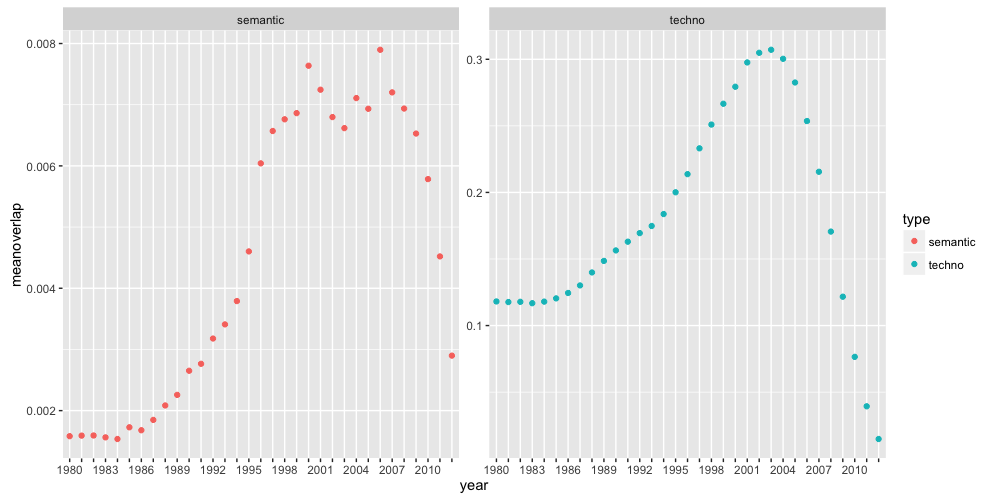
\includegraphics[width=0.49\textwidth]{figures/real_all_ts} 
%\\
%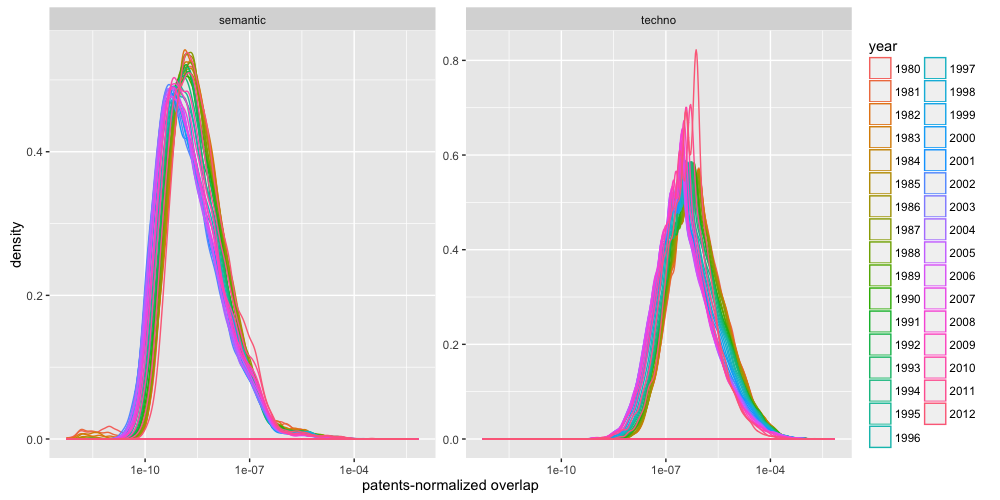
\includegraphics[width=0.49\textwidth]{figures/patentnorm_all_density_logscale}
%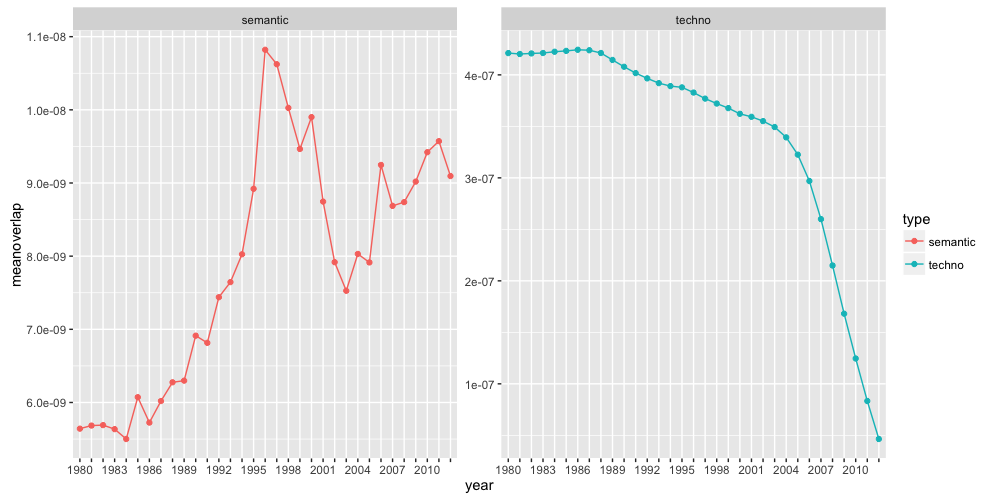
\includegraphics[width=0.49\textwidth]{figures/patentnorm_all_ts} \\

%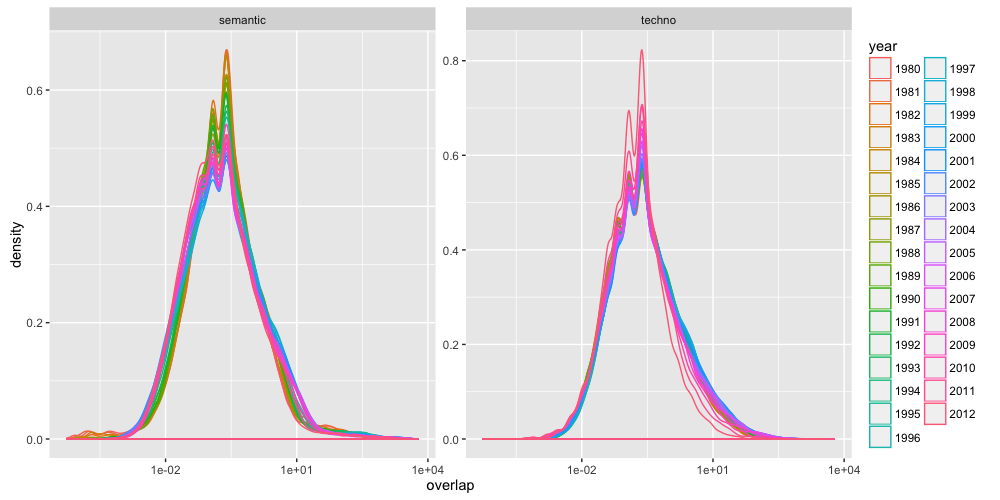
\includegraphics[width=0.49\textwidth]{figures/real_all_density_semcounts}
%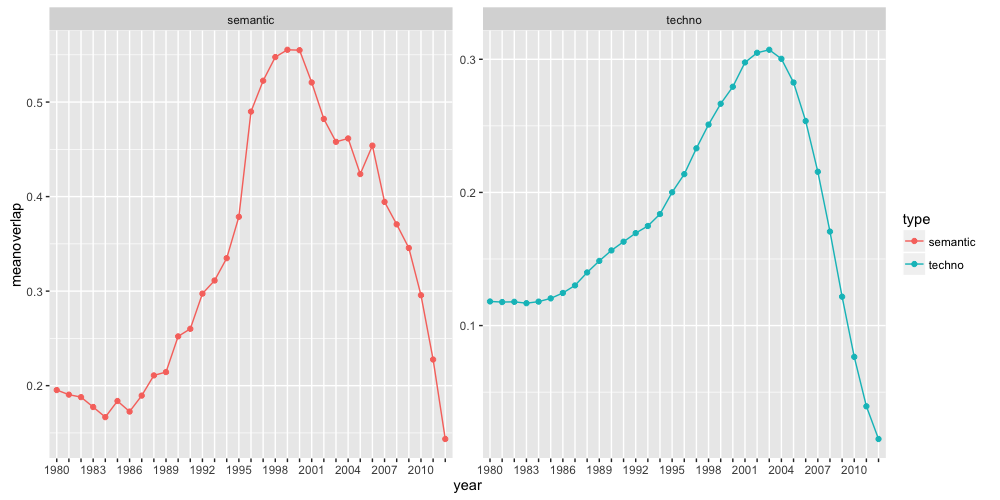
\includegraphics[width=0.49\textwidth]{figures/real_all_ts_semcounts} \\

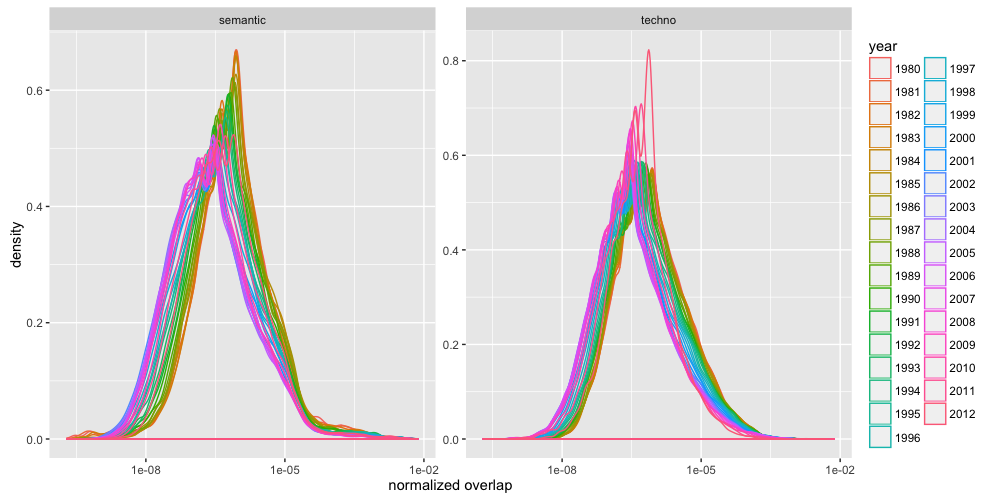
\includegraphics[width=0.49\textwidth]{figures/patentnorm_all_density_semcounts}
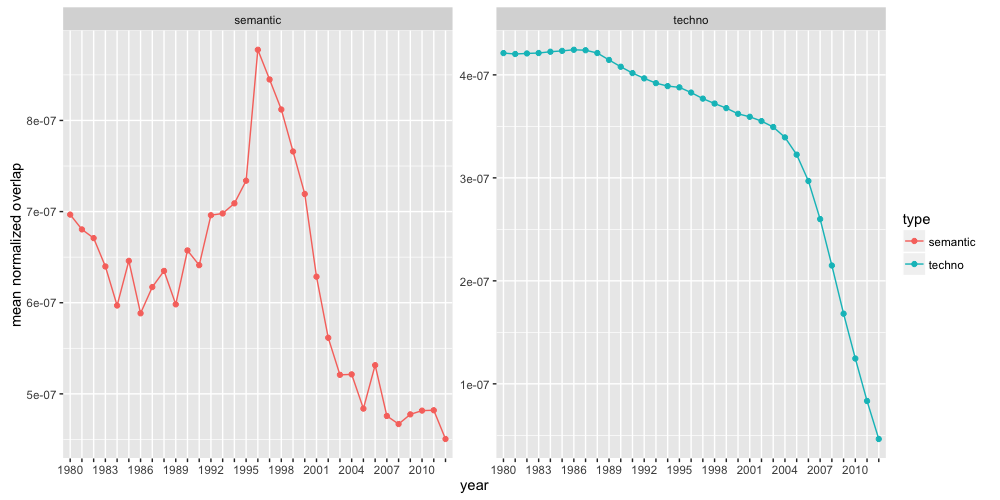
\includegraphics[width=0.49\textwidth]{figures/patentnorm_all_ts_semcounts} \\
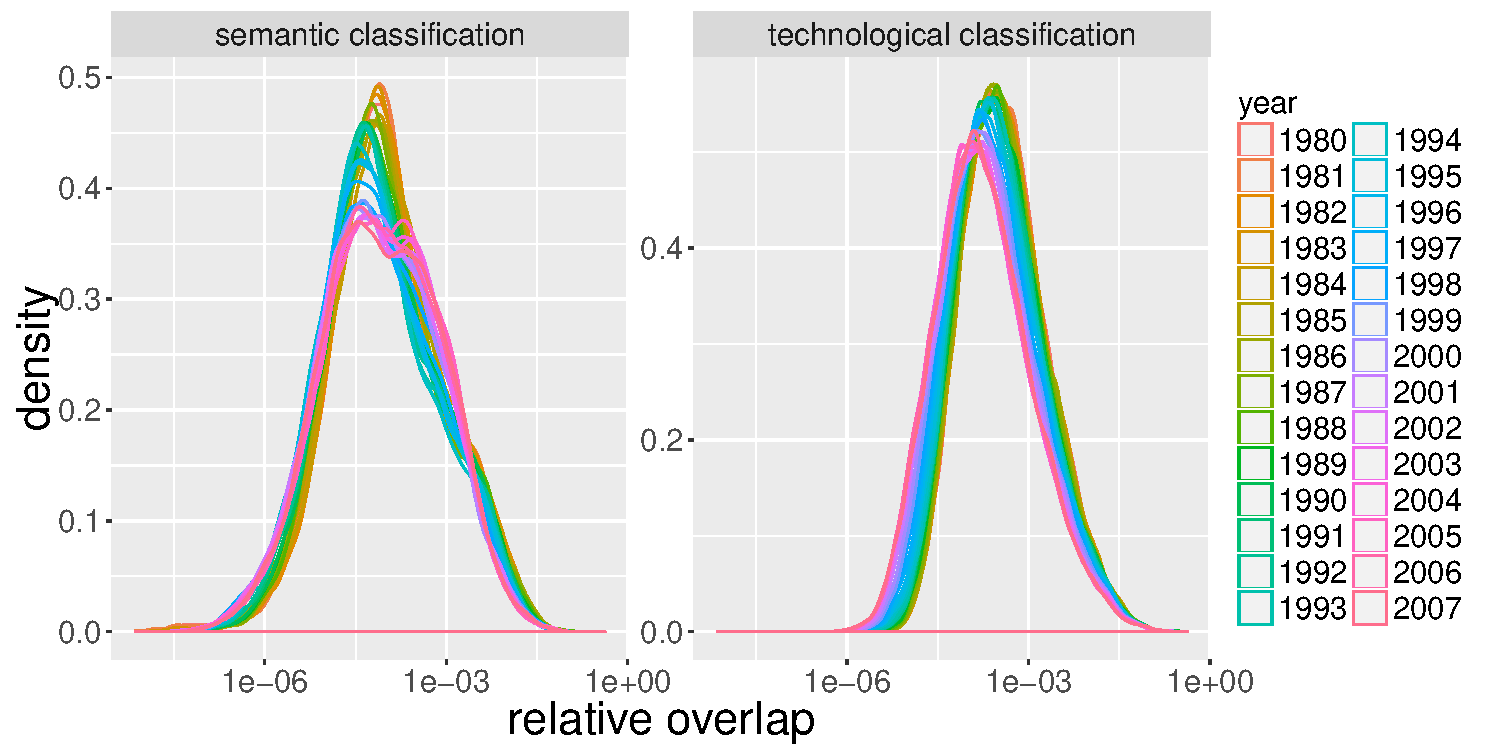
\includegraphics[width=0.49\textwidth]{figures/relative_all_density_semcounts}
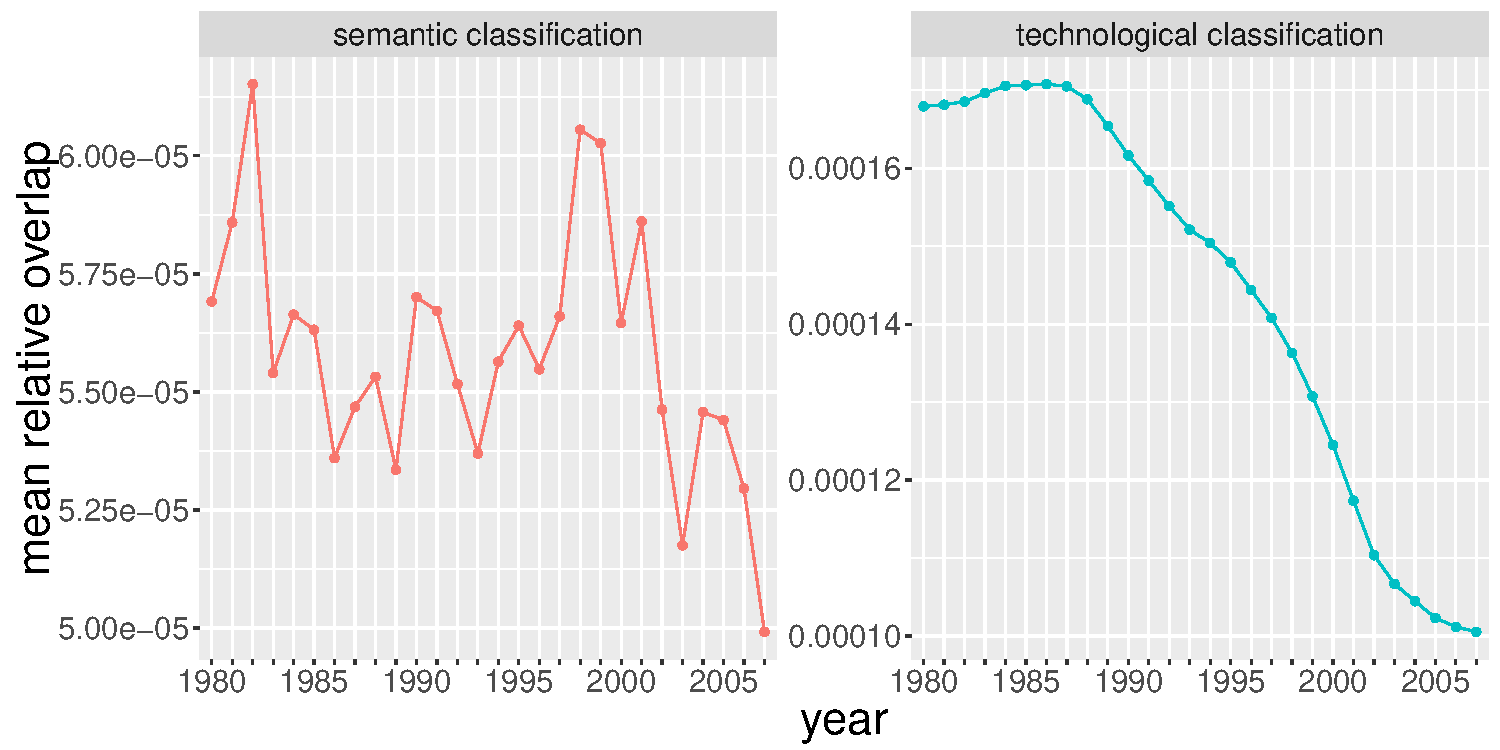
\includegraphics[width=0.49\textwidth]{figures/relative_all_ts_semcounts} 

\caption{
\textbf{Intra-classification overlaps.}
\textit{(Left column)} Distribution of overlaps ($O_{ij}$ for all $i\neq j$; zero are removed because of the log-scale). \textit{(Right column)} Corresponding mean time-series. \textit{(First row)} Normalized overlaps. \textit{(Second row)} Relative overlaps.}
%\comment{(Juste) I put results for different definitions of overlap, which having its sense ; do we choose the most interesting ? (!! selection bias) - First row : non-normalized overlaps, biased by patent count, nothing to say ; Second row : overlaps normalized by patent count - I think there is signal here ; Third-Fourth raw : same plots with semantic probas computed with the number of relevant keywords and not all (removes a "patent-size" effect) ; Fifth row : relative overlaps (jaccard similarity), also with count probas; Note : for log-scale plots, zeros are removed}
\label{fig:intra-classif-overlap}
\end{figure}
%%%%%%%%%%%%%%%%%%%%%%


\paragraph{Inter-classification overlaps}

\comment{Yo: pourrais-tu donner la definition ?}[en fait la def des overlap en debut de section vaut pour le intra et inter, c'est pas clair ?]\comment{Yo:Non, c'est pas clair pour moi le lien.} Overlaps \emph{between} classifications describe their relative correspondence and are a good indicator to spot relative changes, as shown in Fig.~\ref{fig:inter-classif-overlap}. Mean inter-classification overlap clearly exhibits two linear trends, the first one being constant from 1980 to 1996, followed by a constant decrease. Although difficult to interpret directly, this stylized fact clearly unveils a change in the \emph{nature} of inventions, or at least in the relation between content of inventions and technological classification (as we observe a relative shift, it may have only been the way to classify by the bureau that changed). The tipping point being at the same time as the ones observed in the previous sections, it is probably not a coincidence and all of these would be markers of a hidden underlying structural changes in processes. The economic interpretation is for now left for further theoretical, modeling and empirical work.


%\textbf{we observe here the same ``shock'' in 1996 ; the story is a bit different ; here the plot can be understood as the adequacy between the two classifications (its variation imply a variation in adequacy) ; so if there is really a hidden phenomenon, here it caused a constant decrease in inter-overlap.}


%%%%%%%%%%%%%%%%%%%%%%
\begin{figure}[!ht]
% figure : interlayer overlap
%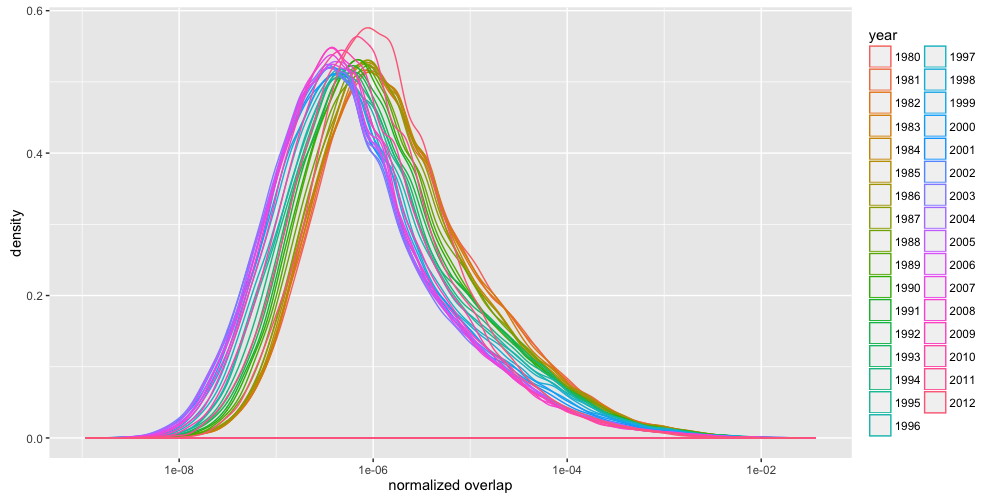
\includegraphics[width=0.49\textwidth]{figures/interov_patentnorm_all_density}
%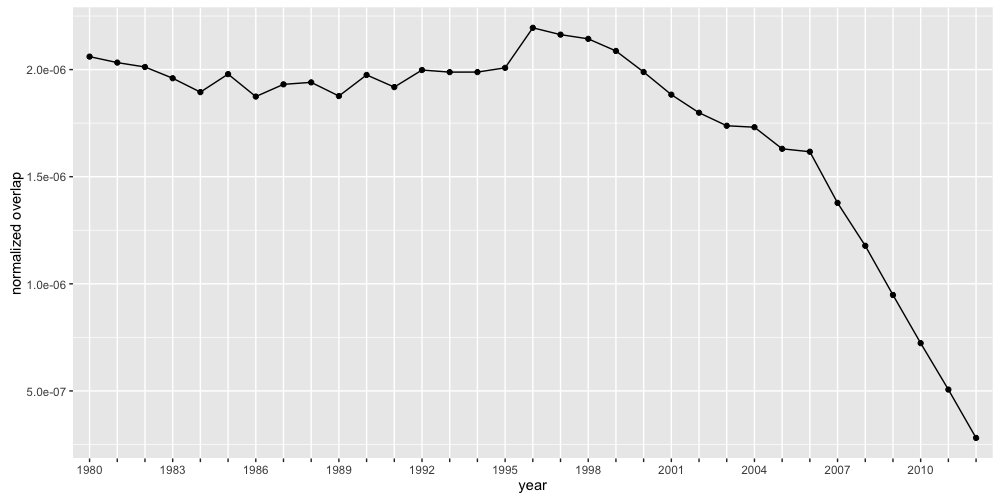
\includegraphics[width=0.49\textwidth]{figures/interov_patentnorm_all_ts}\\

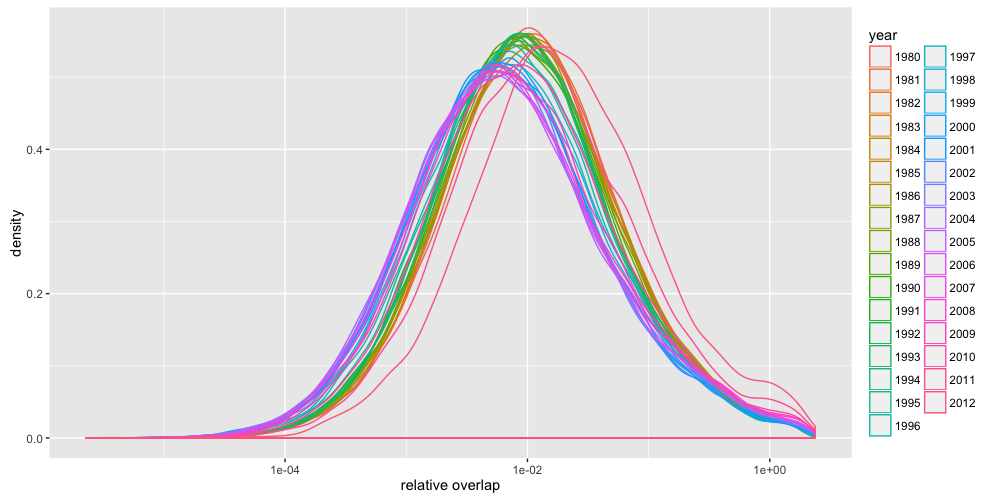
\includegraphics[width=0.49\textwidth]{figures/interov_relative_all_density}
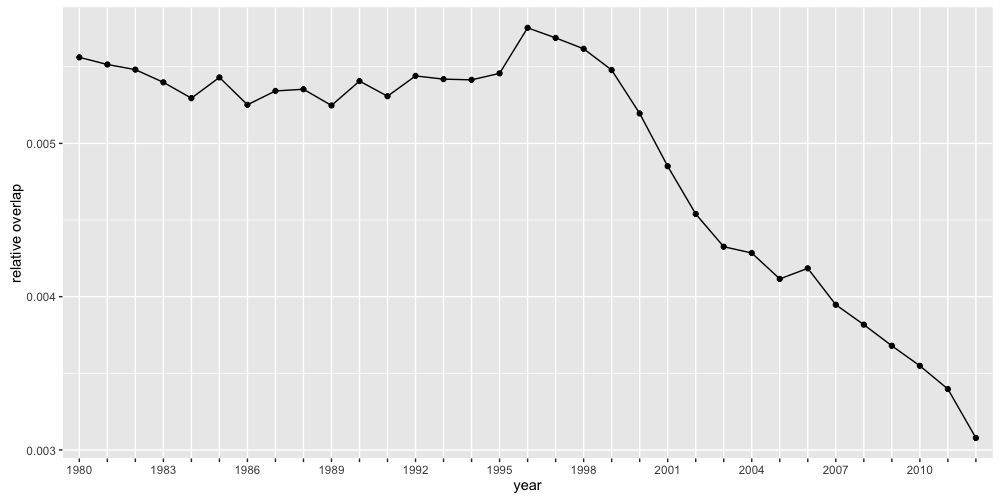
\includegraphics[width=0.49\textwidth]{figures/interov_relative_all_ts}

\caption{\textbf{Distribution of relative overlaps between classifications.} (Left) Distribution of overlaps at all time steps; (Right) Corresponding mean time-series. The decreasing trend starting around 1996 confirms a qualitative regime shift in that period. Effective normalized overlaps (available in Supplementary Material) provide the same qualitative insight.}
\label{fig:inter-classif-overlap}
\end{figure}
%%%%%%%%%%%%%%%%%%%%%%





%%%%%%%%%%%%%%%%%%%%%%
\subsection{Citation Modularity}

%  distribution of second order interdisciplinarity
%   -> in supplementary material ? or is it really necessary ?

%\textbf{I think the heatmaps are not a good idea ; we do not see anything ; I will do the second-order diversity distributions plots but it will be boring to have analog plots as previous sections ; maybe put them in supplementary material ; a good compromise would be the evolution of overlapping communities citation modularity in time, for semantic and techno ; to be linked with Yo's part ; need to code it \cite{nicosia2009extending} and do the plots ; ETA:JR:0.5d}

An exogenous source of information on relevance of classifications is the citation network described in Section \ref{sub:citation}. The correspondance between citation links and class belonging should provide a measure of accuracy of classifications, in the sense of an external validation since it is well-known that citation homophily \comment{def?}[ce n'est pas une mesure particulière, mais une façon de dire que tu cites tes semblables] is expected to be quite high (see, e.g, ~\cite{AAKnetwork2016}). This section studies empirically modularities of the citation network regarding the different classifications, whereas the same aspect will be investigated more rigorously by modeling from a statistical point of view in the next section. Modularity is a simple measure of how communities in a network are well clustered (see \cite{clauset2004finding} for the precise definition). Although initially designed for single-class classifications, this measure can be extended to overlapping classes (when nodes can belong to several classes at the same time, in our case with different probabilities) as introduced by~\cite{nicosia2009extending}. \textcolor{blue}{Super solide ta def Juste, je me suis permis de la solidifier encore pluset je laisse mes commentaires}
\comment{The Simple directed modularity is given in our case by $Q_d = \frac{1}{N_P}\sum_{1\leq i,j\leq N_P}\left[A_{ij} - \frac{k_{i}^{in}k_{j}^{out}}{N_P}\right]\delta(c_i,c_j)$, with $A_{ij}$ the citation adjacency matrix (i.e. $A_{ij} = 1$ if there is a citation from the $i$th patent to the $j$th patent, and $A_{ij}=0$ if not --c'est bien la def que tu avais en tete Juste???), $k_i^{in}$ (resp. $k_i^{out}$) in-degree (resp. out-degree) of patents (i.e. the number of citations from the $i$th patent and the number of citations made to the $i$th patent --- c'est bien ca???) and $c_i$ is defined as the main patent class, which is taken as the primary class for technological classification and the class with the biggest probability for semantic classification. Multi-class modularity is given by $Q_{ov} = \frac{1}{N_P} \sum_{c\in C} \sum_{1\leq i,j \leq N_P}\left[F(p_{ic},p_{jc})A_{ij} - \frac{\beta_{i,j,c}^{out}k_i^{out}\beta_{i,j,c}^{in}k_j^{in}}{N_P}\right]$ where $\beta_{i,j,c}^{out} = \frac{\sum_j F(p_{ic},p_{jc})}{N_P}$ and $\beta_{i,j,c}^{in} = \frac{\sum_i F(p_{ic},p_{jc})}{N_P}$. We take $F(p_{ic},p_{jc}) = p_{ic}\cdot p_{jc}$ as it is suggested in \cite{nicosia2009extending}.}
We show in Fig.~\ref{fig:modularities} both simple and multi-class modularities in time. For simple modularity, technological classification is low and stable whereas semantic is slightly greater and increasing (expect perturbations in latest years that should be due to the non-stationarity of citation processes). These values are however low and suggest that single classes are not enough to capture citation homophily. Multi-class modularities tell a totally different story. First of all, both classification modularities have a clear increasing trend, meaning that they are in time more and more adequate with citation network. This effect could have been expected regarding the specializations unveiled in previous subsections. Secondly, semantic modularity dominates technological modularity by an order of magnitude (e.g. 0.012 against 0.082 in 2010) at each time. Quantitatively not interpretable, this discrepancy has a strong qualitative significance: our semantic classification is much more adequate to the citation network when using multiple class. This underlines one of the advantages of our classification approach, that is the ability to take fully into account the heterogeneous nature of invention through this multi-class aspect. \comment{la derniere phrase est pas claire, et de plus on n'a plus au vu des plots l'originalite semantic ne monte pas, si?}[je vais reformuler, ce que je voulais dire c'est l'exemple de la figure ci-dessous]




%%%%%%%%%%%%%%%%%%%%%%
\begin{figure}[!ht]
\centering
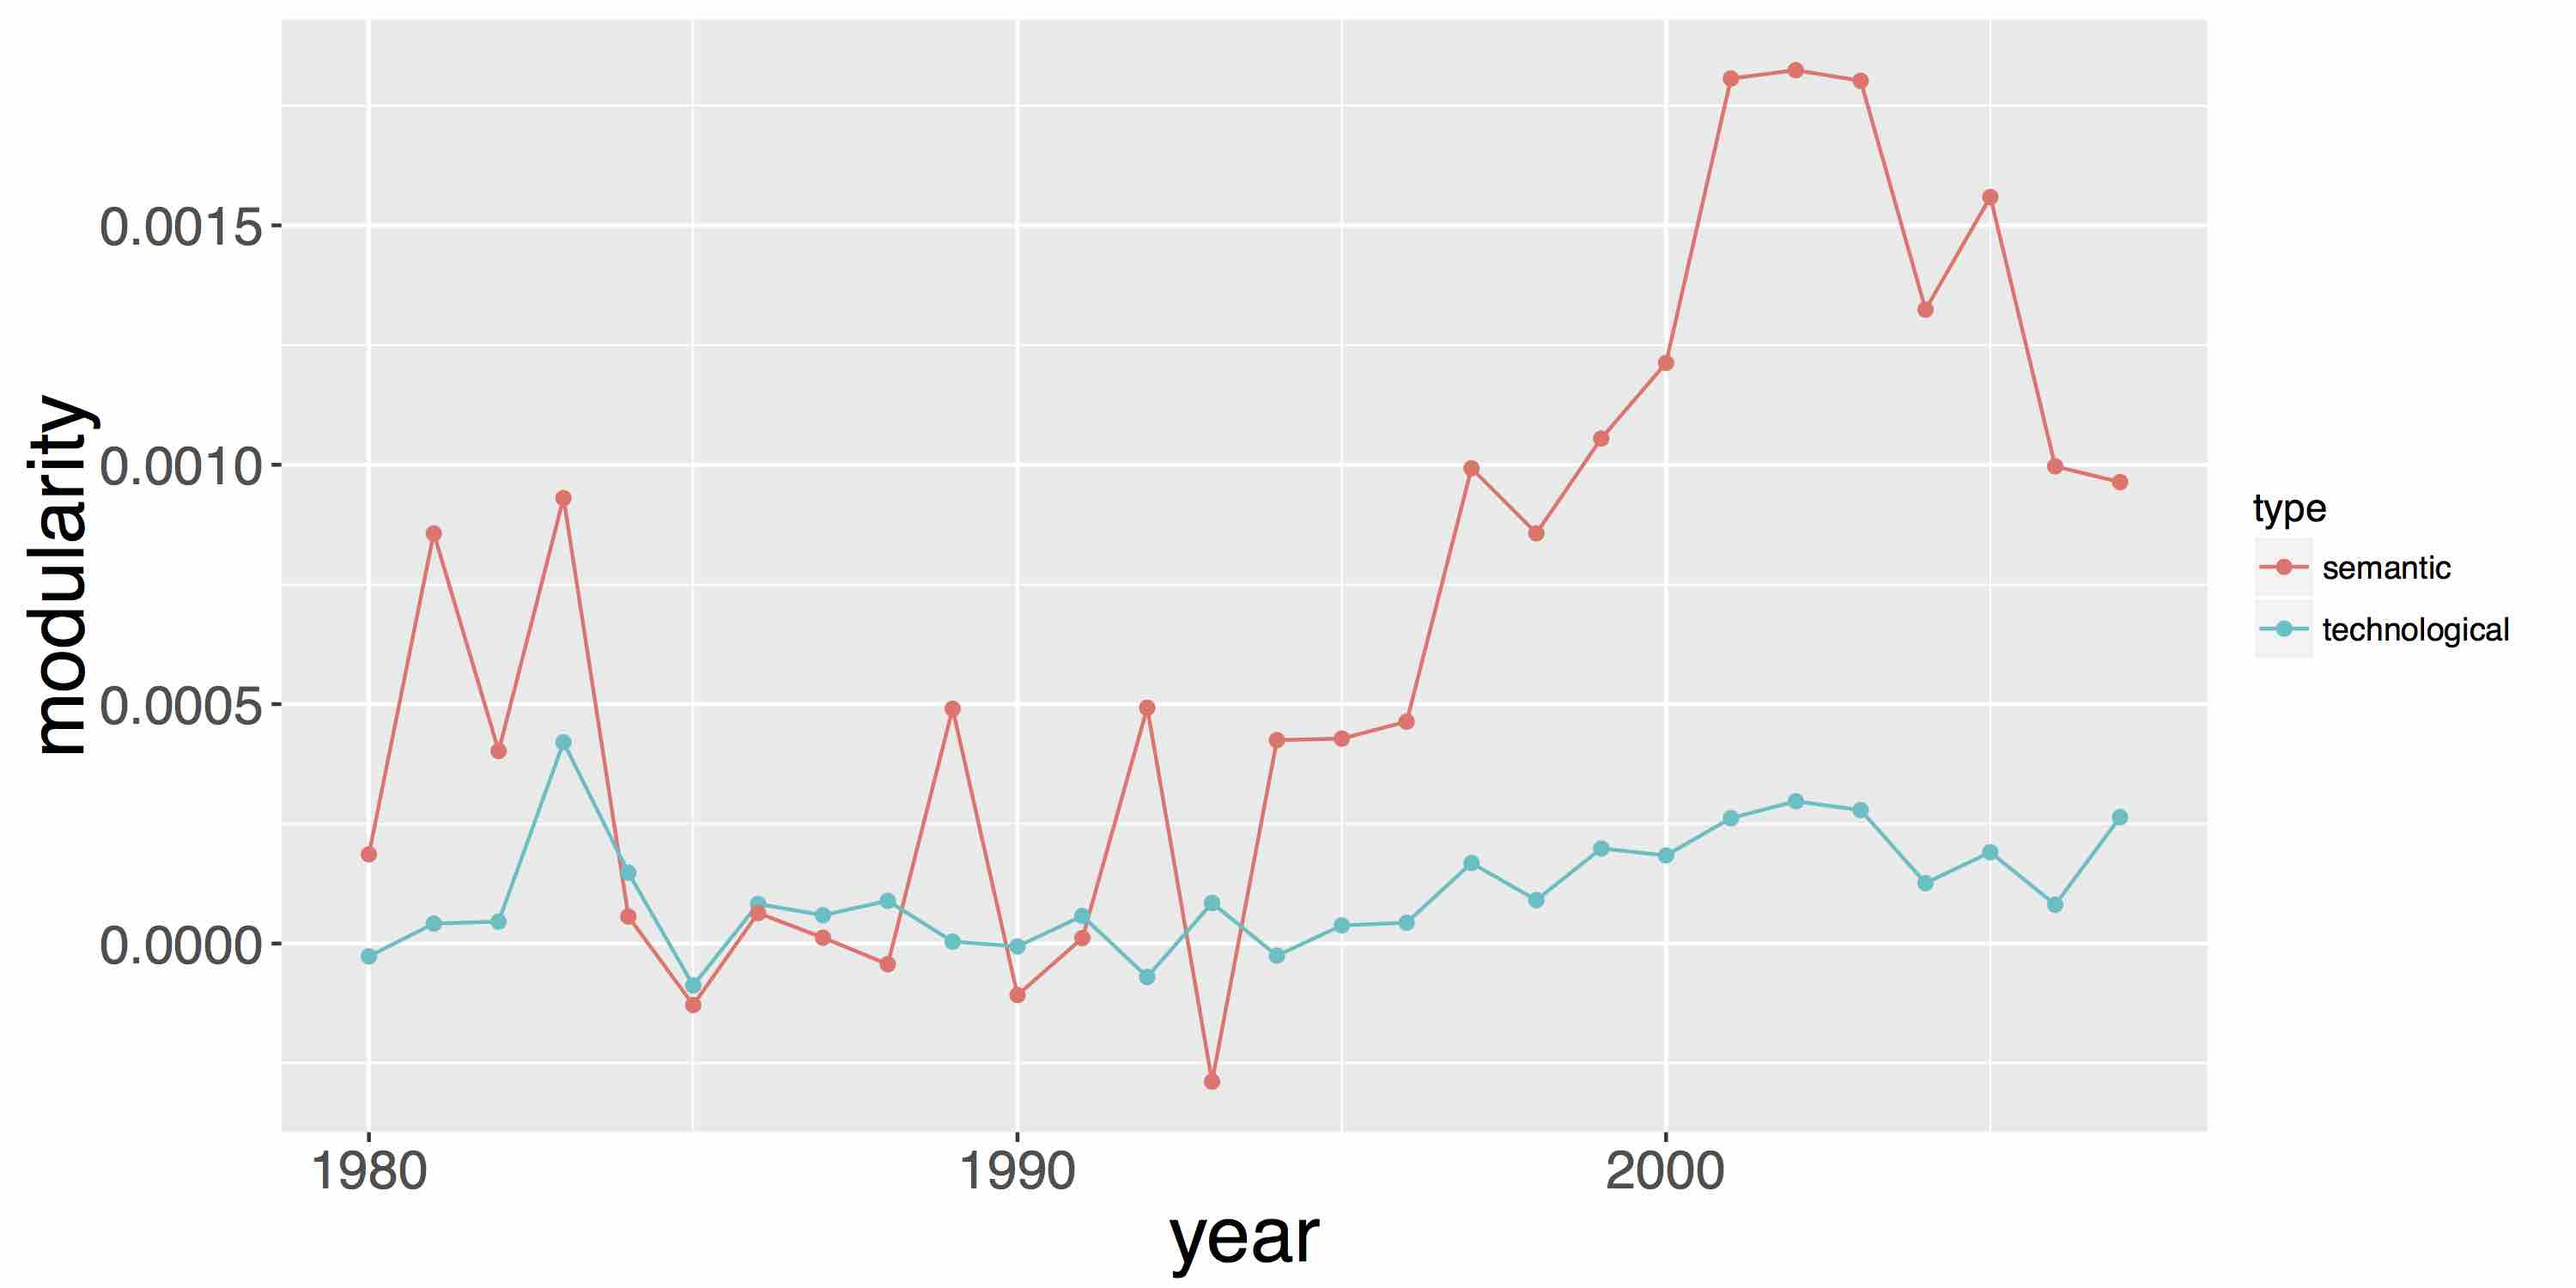
\includegraphics[width=0.49\textwidth]{figures/simplemodularity}
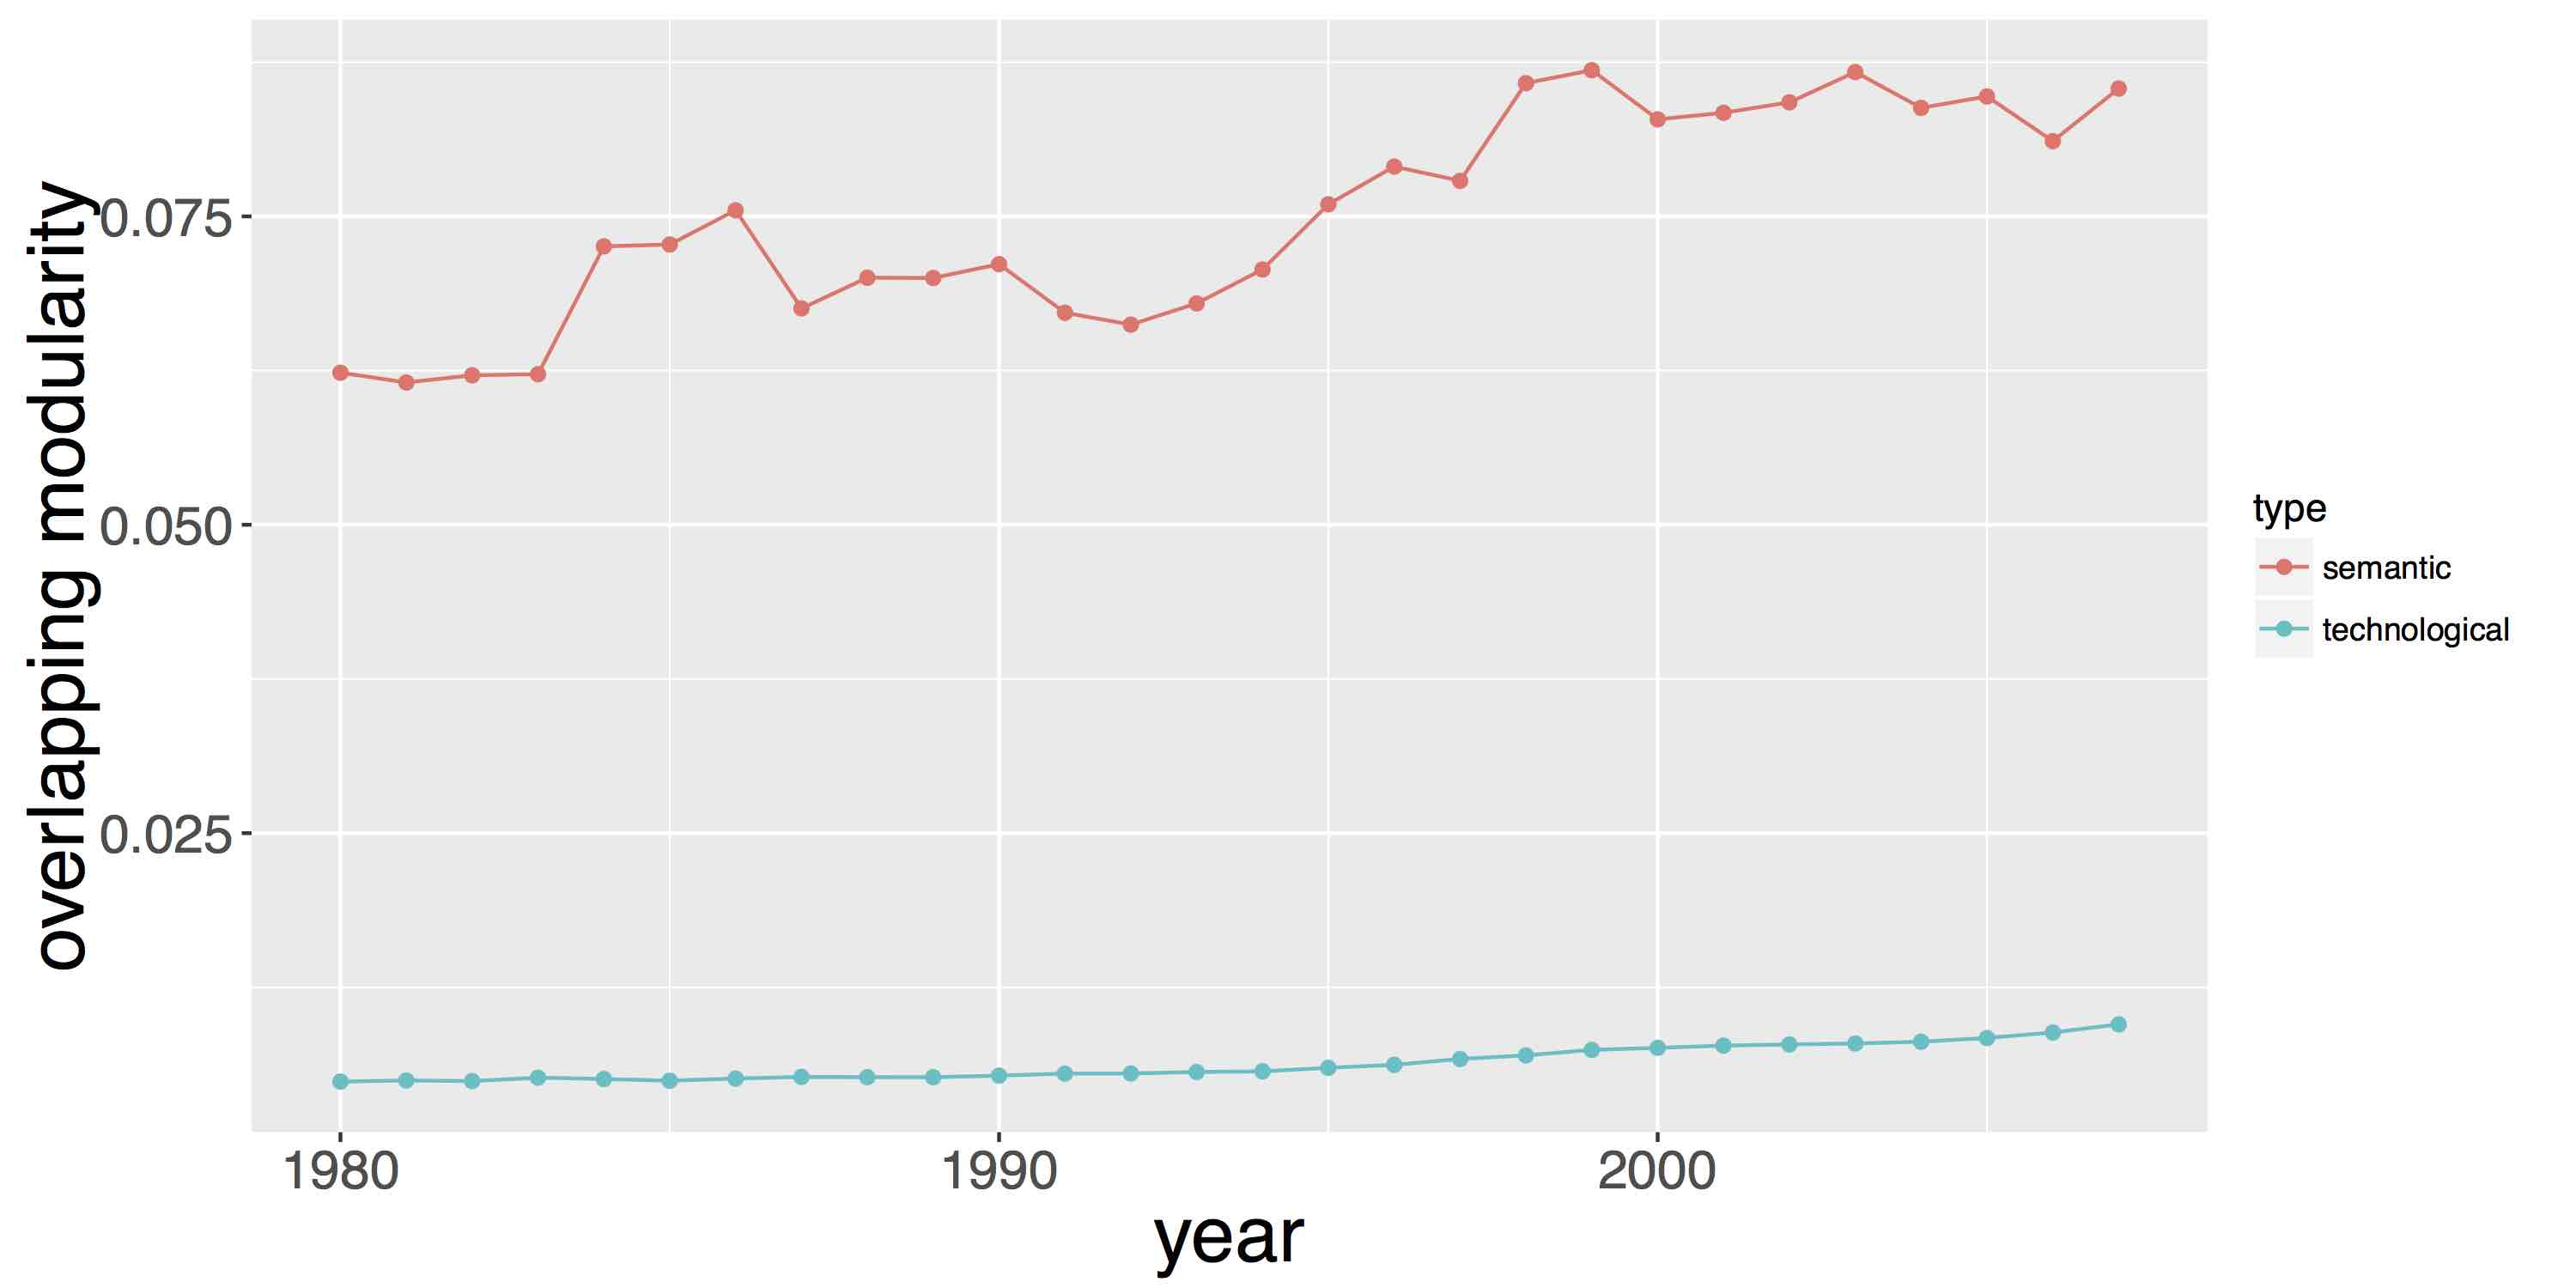
\includegraphics[width=0.49\textwidth]{figures/overlappingmodularity}
\caption{\textbf{Temporal evolution of semantic and technological modularities of the citation network.} (Left) Simple directed modularity, computed with patent main classes (main technological class and semantic class with larger probability). (Right) Multi-class modularity, computed following~\cite{nicosia2009extending} \comment{Yo: pourquoi les derniers points sont variables comme ca a gauche? c'est quoi la difference entre les deux def ?}[la variabilité je me disais que ça devait être du au fait que le regime de citation est pas encore stationaire pour les dernieres années, du coup elles apparaissent plus comme random ; mais pourquoi ça arrive moins sur techno (un peu comparé à la faible variabilité dans le temps), et pas avec la multi-class, difficile à savoir - ça doit vouloir dire que la destabilisation due aux citations manquantes se reporte sur des classes voisines (en terme d'overlap) ce qui ne modifie pas la multi-class modularity. La diff entre les deux, la première suppose une unique classe par patent, la deuxième prend en compte les probabilités des patent d'appartenir aux classes : si un patent 55\% x et 45\% y cite 50\% de x et 50\% de y, avec la modularité simple le lien y-y assez fort ici est ignoré, avec la deuxième il est pris en compte]}\comment{ok t'as l'air cale dessus, pas forcement besoin de commenter, mais on peut peut etre retirer les dernieres annees en disant qu'elles sont bruitees!}
\label{fig:modularities}
\end{figure}
%%%%%%%%%%%%%%%%%%%%%%














%%%%%%%%%%%%%%%%%%%%%
\subsection{Statistical Model}
\label{statisticalmodel}
\textcolor{red}{Je pense que le premier paragraphe peut etre mis avant la methode de Juste, car fondamentalement c'est le meme genre de trucs qui est fait (si je ne m'abuse pas!)}  
In this section, we develop a statistical model aimed at quantifying performance of both technological and semantic classification systems.
\textcolor{green}{The inclusion of 'perform' in the previous sentence is perhaps a little rash. It is not the point to show that one approach dominates the other, but rather than our new approach enjoy good statistical properties.} \textcolor{red}{je trouve cette formulation un peu malvenue pour un papier scientifique ; est-ce qu'on pourrait remplacer par un truc comme (bien reformulé du coup) ``\ldots classification systems, in the sense that an external validation of classifications and a statistical comparison, with the inclusion of the citation network.''}

To compare the technological and semantic classes, we choose to look at within class citations proportion (for both technological and semantic approaches). We provide two obvious reasons why we choose this. First, the citations are commonly used \textcolor{red}{shall we make some citations here, or refer to the introduction?} as a proxy for performance. Second, this choice is "statistically fair" in the sense that both approaches have focused on various goals and not on maximizing directly the within class proportion. 
Nonetheless, the within class proportion is too sensitive to the distribution of the shape of classes. For example, a dataset where patents for each class account for 10\% of the total number of patents will mechanically have a better within class proportion than if each class accounts for 1\%. Consequently, an adequate statistical model, which treats datasets fairly regardless of their distribution in classes, is needed. 

We introduce a simple model of citations network growth conditional to a classification, which can be expressed as a stochastic block model (e.g. \cite{decelle2011asymptotic}, \cite{valles2016multilayer}), and compute the corresponding maximum likelihood estimator (MLE). In view of~\cite{2016arXiv160602319N}, this can be thought as equivalent to maximizing modularity measures.

To compare both approaches, a formal definition of the problem is needed. In addition, models for both approaches are required. We need to introduce some notations to answer those two questions. We consider a specific window of observations (typically 5 years long), and we define $Z$ the number of patents which appeared during that time window. We let $t_1, \cdots, t_Z$ their corresponding appearance date by chronological order. For each patent $i=1, \cdots, Z$ we consider $C_i$ the number of distinctive couples \{cited patent , cited patent's class\} made by the $i$th patent (for instance if there is only one citation and that the cited patent is associated with three classes, then $C_i = 3$). Let $z \in \{tec, sem\}$, which stands respectively for "technological class" and "semantic class". We define $N_{k,i}^{(z)}$  the number of patents associated to the $k$th technological or semantic class at the time of the $i$th patent's submission. Correspondingly, we define as
$$S_i^{(z)} = \sum_{k \geq 1} N_{k,i}^{(z)}$$
the sum of patents' number of classes at time $t_i$. For $l = 1, \cdots, C_i$ we consider the Bernoulli variables $B_{l,i}$, which equal $1$ if the cited patent's class is also common to the $i$th patent. We assume that $B_{l,i}$ are independent of each other and follow 
$$B \Big( \min \Big\{ 1, \frac{\sum_{k \in K_{i}} N_i^{(z)}}{S_i^{(z)}} + \theta^{(z)} \Big\} \Big),$$ 
where $K_i$ corresponds to the ith patent classes. The parameter $0 < \theta^{(z)} < 1$ indicates the propensity for any patent to cite patents of its own technological or semantic class. When $\theta^{(z)} = 0$, the probability of citing patents from its own class is simply $\frac{\sum_{k \in K_{i}} N_i^{(z)}}{S_i^{(z)}}$ , which is what we would have if classes were assigned randomly and independently from patents' contents. Conversely, there are 100\% of within class citations when $\theta^{(z)} = 1$. Finally, we assume that the number of couples $C_i$ are a sequence of independent and identically distributed random variables following the discrete distribution $C$, and also independent from the other quantities.

The problem can now be expressed as the statistical test $\theta^{(sem)} > \theta^{(tec)}$. To do that, we first estimate $\theta^{(z)}$ via maximum likelihood, and obtain the corresponding MLE $\hat{\theta}^{(z)}$. The likelihood function, along with derivations of the standard deviation expression and details about the test, can be found in Supplementary Material \textcolor{red}{C'est bien comme ca qu'on appelle l'Appendix?}. The fitted values, standard errors, statistic values and p-values on non-overlapping blocks from the period 81-2010 are reported on Table bla bla. We use different values of thresholds for semantic classes. For a given class and threshold, we only keep the patents with a semantic value \textcolor{red}{Comment t'appelles ca Juste?}\textcolor{blue}{tu peux mettre ``semantic probability'', c'est exactement la proba empirique du patent d'appartenir à la classe} above the threshold. Bla bla ba to continue on interpretation








%%%%%%%%%%%%%%%%%%%%%
\section{Discussion \label{discussion}}
%%%%%%%%%%%%%%%%%%%%%

% Rationale for now : extract information that is quite independent from technological classification ; potential of this method demonstrated through simple examples (descriptive stats, basic measures, simple model)

% develop here the possible developments we talked about (trajectories of firms, etc ?)



%%%%%%%%%%%%%%%%
\subsection{Further Developments}

%%%%%%%%%%%%%%%%%%%%%
\paragraph{Supervised and unsupervised Data Mining}

% learn patterns, what makes a patent innovative ; detect breakthrough innovation, etc.

We tested simple potential predictors of patent innovative character and/or success, i.e. supervised data-mining. \comment{Anto put here your regressions, to demonstrate the potentialities of our approach as predictors ?}

Insights from unsupervised data-mining techniques on features linked to both classifications, patents characteristics and the citation network, will surely be a broad and fertile research direction to investigate. As this kind of approach generally requires a fine-tuning of features (at least with ``classical'', non-deep, techniques) that could be the subject of a full paper, we let this for further work.



%%%%%%%%%%%%%%%%%%%%%
\paragraph{Multi-modeling semantic classification}

The semantic classification method could be reinforced by combining it with other techniques such as Latent Dirichlet Allocation which is a widely used topic detection method~\cite{blei2003latent}, already used on patent data as in~\cite{kaplan2015double} where it provides a measure of idea novelty and the counter-intuitive stylized facts that breakthrough invention are likely to come out of local search in a  field rather than distant technological recombination. Using this approach should first help further evaluate the robustness of our qualitative conclusions (external validation), and secondly, depending on the level of orthogonality with our classification, potentially bring an additional feature to characterize patents, in the spirit of multi-modeling techniques where neighbor models are combined to take advantage of each point of view on a system.


%%%%%%%%%%%%%%%%%%%%%
\paragraph{Hyper-network analysis}

% how different info layers : citations ; techno ; semantic forms a multiplex (nodes = patents, with different types of connexions)

% we can then use multi-layer network analysis, such as generalized centrality de la miss Elisa \cite{de2015ranking}

%\textbf{how bipartite/multilayer approaches can push us further ; ex multilayer centrality that is trendy and hot now~\cite{de2015ranking} %(as the miss working on it ---> https://twitter.com/elisa_omodei ;) - totally unscientific sorry, it's to see if you read the comments ^^)

% note : redefine more precisely layers of the nw and clarify if dealing with multilayer nw or hypernw. if nodes are patents only, that can be linked by different type of relations (citation, belonging to same techno class, belonging to same semantic class) then it is an hypernetwork.

%\cite{iacovacci2015mesoscopic} provide a method to compare macroscopic structures of the different layers in a multilayer network. We apply a similar methodology to compare technological and semantic layers.

Our use of network analysis stayed somehow limited here, and newly developed techniques could be applied. Indeed, patents and keywords can for example be nodes of a bipartite network, or patents be links of an hyper-network, in the sens of multiple layers with different classification links and citation links. \cite{iacovacci2015mesoscopic} provide a method to compare macroscopic structures of the different layers in a multilayer network, what could be applied as a refinement of the overlap, modularity and statistical modeling done here. Furthermore, is has been recently shown that measures on projections of multilayer networks induced a significant loss of information compared to the generalized corresponding measure~\cite{de2015ranking}, what confirms the potentiality of such a development.





%%%%%%%%%%%%%%%%%%%%%
\paragraph{Towards a more exhaustive database}

%\textit{how we will parse full texts ; do OCR (we won't, we will parse Google as it would take at least a postdoc to manage a very bad OCR, whereas gogole is an easy target with very good data ; the difficult point will be to explain how we actually got the data...)}

\comment{Attention, un peu contradictoire avec la partie "toward a complementary classification}
Our semantic analysis was limited to the text of abstracts and a legitimate question is what information the use of full texts would allow to capture: it may contain more information but with more noise, making the filtration process more tricky; it may also be less structured than abstracts and thus have a smaller information-to-length ratio (compression rate) than using abstracts. These questions can not be answered from scratch, as the level of compression and information loss of the abstract writing process is not known. USPTO redbook raw data provides full texts up to 1976: their collection will be a first step into the reinforcement of our database. \comment{Je préfère séparer bien les choses, ici on parle de récupérer les full texts, plus loin on parle de remonter plus loin dans le temps. Donc je déplacerai la phrase suivante}. Furthermore, going back in time, patents are available in image format. Then the use of Optical Character Recognition techniques is a way to retrieve plain text and extend our analysis in time, with both abstracts and full texts.

\comment{Les gars là-dessus j'ai trouvé la pirouette pour qu'on s'en sorte : on va crawler google, faire l'extended database, et la poster sur dataverse de manière anonyme (compte anonyme, faux nom et independent researcher, tout ça derrière ip anonyme), on aura plus qu'à la recup et la citer pour l'utiliser ! :) }[Pour une prochaine application alors ?]




%%%%%%%%%%%%%%%%%%%%%
\subsection{Potential Applications}

% I put random ideas ; plan not fixed at all !


%%%%%%%%%%%%%%%%%%%%%
\paragraph{Trajectories of firms}

\comment{En chantier}[][]

The existence of a classification for technology enables researchers to build a technology space in which each USPC class is an axis. This approach has been popularized by~\cite{Jaffe1986distance} and is namely used in~\cite{Bloom2005distance} to consider firms' technological proximity. This approach has also been used to study the existence of clusters of technology or knowledge spillover. In our framework, we add an additional classification whose construction does not directly rely on the USPC system. It is therefore possible to use the current firm's patents portfolio and its content in terms of semantic class to study its movement in a technological space.~\cite{omodei2014social} studies trajectories of authors in a semantic space.



%%%%%%%%%%%%%%%%%%%%%
\paragraph{Towards concrete measures of endogenous growth theories}

\textit{recall the very beginning of the project ; Aghion et al. ; is it a good idea Anto ?}


%%%%%%%%%%%%%%%%%%%%%
\paragraph{Looking backward into the history of innovation}

USPTO patent data have been digitized from the first patent in July 1790. However, not all of them contain a text that is directly exploitable. We consider that the quality of patent's images is good enough to rely on Optical Character Recognition techniques to retrieve plain text from at least 1920. With such data, we would be able to extend our analysis further back in time and to study how technological progress occur and combine in time. ~\cite{akcigit2013mechanics} conduct a similar .



%%%%%%%%%%%%%%%%%%%%%
\section{Conclusion}




%%%%%%%%%%%%%%%%%%%%%
\section*{Supporting Information \label{sectionSI}}
% Include only the SI item label in the subsection heading. Use the \nameref{label} command to cite SI items in the text.

\subsection*{S1 Text : Definition of utility patent}

\textbf{Describes with more details the definition of patents and  context.}

\subsection*{S2 Text : Data collection procedure}

\textbf{Detailed description of data collection}

\subsection*{S3 File : Semantic Network Visualization}

\textbf{Vector file of the semantic network (Fig.\ref{fig:rawnetwork})}




%%%%%%%%%%%%%%%%%%%%%
%\section*{Acknowledgments}





\nolinenumbers

%\section*{References}
% Either type in your references using
% \begin{thebibliography}{}
% \bibitem{}
% Text
% \end{thebibliography}
%
% OR
%
% Compile your BiBTeX database using our plos2015.bst
% style file and paste the contents of your .bbl file
% here.
% 


\bibliographystyle{plos2015}
\bibliography{patents}




%%%%%%%%%%%%%%%%%%%%
%% Supplementary Information
%%%%%%%%%%%%%%%%%%%%


\newpage

\section*{Supporting Information \label{sectionSI}}

\subsection*{Definition of utility patent} 

A utility patent at the USPTO is a document providing intellectual property and protection of an invention. It excludes others to making, using, or selling the invention the same invention in the United States in exchange for a disclosure of the patent content. The protection is granted for 20 years since 1995 (it was 17 years before that from 1860) starting from the year the patent application was filled, but can be interrupted before if its owner fails to pay the maintenance fees due after 3.5, 7.5 and 11.5 years. Utility patents are by far the most numerous, with more than 90\% of the total universe of USPTO patents.\footnote{Other categories are Plant patents, Design patents and Reissue patents.} According to the Title 35 of the United States Codes (35 USC) section 101: \textit{``Whoever invents or discovers any new and useful process, machine, manufacture, or composition of matter, or any new and useful improvement thereof, may obtain a patent therefor, subject to the conditions and requirements of this title.''}\footnote{%
Patent laws can be found in http://www.uspto.gov/web/offices/pac/mpep/mpep-9015-appx-l.html\#d0e302376} In practice however, other types of invention including algorithms can also be patented.\footnote{A notable example is the patent \textit{US6285999} protecting the Page Rank algorithm invented by Larry Page in 1998 which was the genesis of Google.} The two following sections of the 35 USC defined the condition an invention must meet to be protected by the USPTO: (i) novelty: the claimed invention cannot be already patented or described in a previous publication (35 USC section 102); (ii) obviousness: \textit{``differences between the claimed invention and the prior art must not be such that the claimed invention as a whole would have been obvious before the effective filing date of the claimed invention to a person having ordinary skill in the art to which the claimed invention pertains''}. (35 USC section 103). After review from the USPTO experts, an application satisfying these requirements will be accepted and a patent granted. The average time lag for such a review is on average a little more than 2 years since 1976, with some patents being granted after much more than two years.\footnote{This time lag, sometimes called the grant lag, is highly heterogeneous across technological fields. In addition, it cannot be considered as totally random. For example, if the patent is really disruptive some competitors might have some incentive in delaying the process by disputing the validity of the patent, for more details see~\cite{regibeau2010}.}


\paragraph{Sample restriction}
As explained briefly before, we consider every patent granted by the USPTO between 1976 and 2013. For each patent, we gather information on the year of application, the year the patent was granted, the name of the inventors, the name of the assignees and the technological fields in which the patent has been classified (we get back to what these fields are below). We restrict attention to patents applied for before 2007. The choice of the year 2007 is due to the truncation bias: we only want to use information on granted patents and we get rid of all patents that were rejected by the USPTO. However, in order to date them as closely as possible to the date of invention, we use the application date as a reference. As a consequence, as we approach the end of the sample, we only observe a fraction of the patents which have been granted by 2013. Looking at the distribution of time lag between application and grant in the past and assuming that this distribution is complete in time, we can consider that data prior to 2007 are almost complete and that data for 2007 are complete up to 90\%.

%%%%%%%%%%%%%%%%%%%%%%%%
\begin{figure}
 %\vspace{1cm}
\centering
\frame{
\includegraphics[scale=0.8]{figures/cit_lag.png}
}
 \caption{Number of citations per lag in year}
 \label{fig1}
\end{figure}
%%%%%%%%%%%%%%%%%%%%%%%%


%%%%%%%%%%%%%%%%%%%%
\subsection*{Data collection procedure}

\label{supp:data}

Raw version of USPTO redbook with abstracts are available for years 1976-2014 starting from bulk download page at \url{https://bulkdata.uspto.gov/}. A script automatically downloads and proceeds files, with the following filters transforming different format and xml schemes into a uniform dictionary data structure :

\begin{itemize}
\item \texttt{dat} files (1976-2000) : handmade parser
\item \texttt{xml}
\end{itemize}

Everything is then stored into a MongoDB database, which latest dump is available at \url{http://dx.doi.org/10.7910/DVN/BW3ACK} % TODO find a way to anonymize the db for submission




%%%%%%%%%%%%%%%%%%%%
\subsection*{Network Sensitivity Analysis \label{app:sensitivity}}

% indicators etc

% sensitivity on time window length ?


\subsubsection*{Network Optimization for all years}

% plots for all years

% TODO plots for all years and pointer here to subfolder on repo ?

The example of Fig.~\ref{fig:networksensitivity} for a given year yielded the same qualitative behavior for all years. All corresponding plots are available on the repository at \texttt{}.




\subsubsection*{An alternative filtering method}

Other heuristic for network construction were tested. We describe one in the following. We assume the highest degree terms do not carry specific information on particular classes and can be thus filtered given a maximal degree threshold $k{max}$. Similarly, edge with small weight must not carry significant information and are filtered according to a minimal edge weight threshold $w_{min}$. Keywords are preliminary filtered by a document frequency window $\left[ f_{min},f_{max} \right]$ which is slightly different from network filtering and complementary. A sensitivity analysis of resulting network topology to these parameters is shown in Fig. .


%%%%%%%%%%%%%%%%%%%%
\begin{figure}[!ht]
% values of some topological measures in 2D parameter space
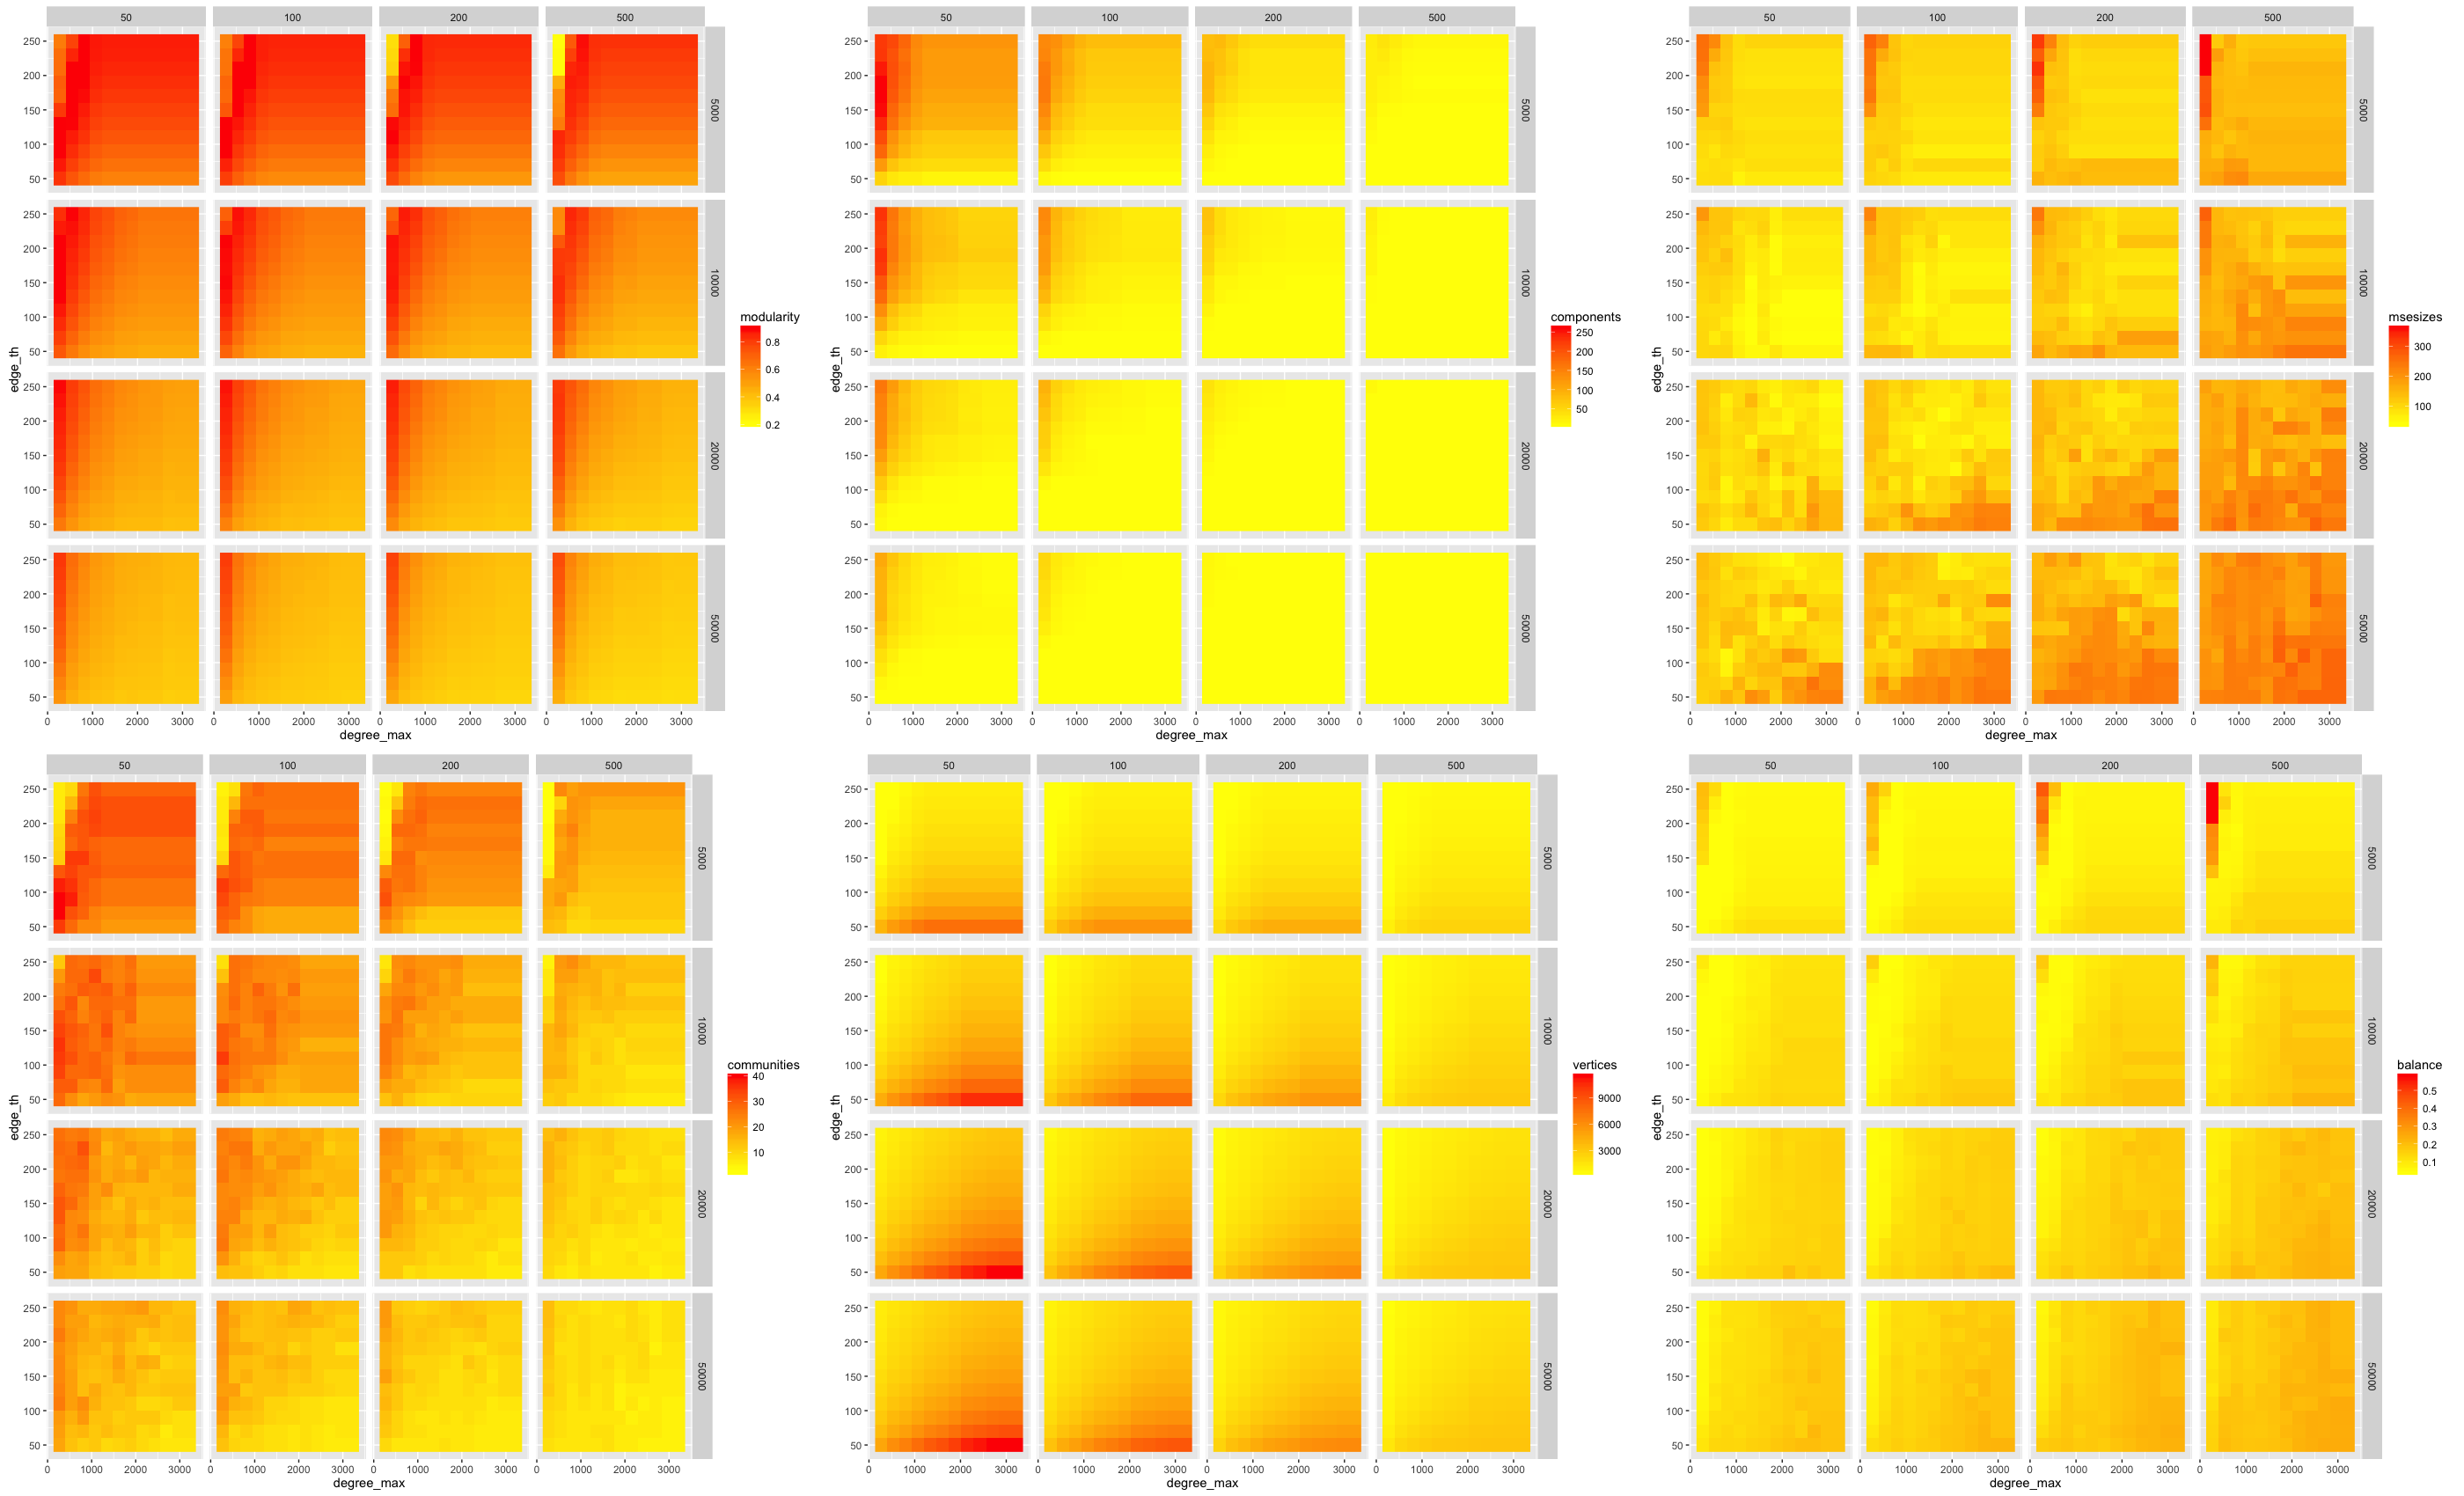
\includegraphics[width=\textwidth]{figures/graph_sens_2010_msesizes}
\caption{Variation of semantic network indicators across a 4-dimensional parameter space (figure-level axis : $(k_{max},w_{min})$; meta axis: $(f_{min},f_{max})$), for year 2010, where indicators are modularity (louvain method), number of connected components, proximity of class size distribution to technological classes size distribution, communities number, network size, community size balance. A good optimization compromise is given here by $()$.}
% TODO change with proportion parameters in new figure
% TODO detail which obj to be minimized etc in supplementary material
\end{figure}
%%%%%%%%%%%%%%%%%%%%


%%%%%%%%%%%%%%%%%%%%
\subsection*{Semantic Network Characteristics}

% network degree distrib, connected components, etc.
% -> basic descriptive stats of the nw

\textcolor{red}{not sure this additional work is very useful}




%%%%%%%%%%%%%%%%%%%%
\subsection*{Time-window size sensitivity}

% put some graphs for 3-years time window : same qualitative properties but a bit more noisy

% TODO which graphs ?










%%%%%%%%%%%%%%%%%%%%
\subsection*{Statistical derivations}
\subsubsection*{Likelihood expression}
This will facilitate the likelihood analysis in the following. We have
\begin{eqnarray*}
\log \mathcal{L} \big( C_N, C_N^{(z)} , \cdots , C_1, C_1^{(z)} \big) & = & \sum_{i=2}^N \log \mathcal{L} \big( C_i, C_i^{(z)} | C_{i-1}, C_{i-1}^{(z)} \cdots , C_1, C_1^{(z)} \big) + \log \mathcal{L} \big( C_1, C_1^{(z)} \big).
\end{eqnarray*}
Note that in view of our assumptions we have
\begin{eqnarray*}
\log \mathcal{L} \big( C_i, C_i^{(z)} | C_{i-1}, C_{i-1}^{(z)} \cdots , C_1, C_1^{(z)} \big) & = & \log \mathcal{L} \big( C_i, C_i^{(z)} | N_{i}^{(z)} \big)\\
& = & \log \mathcal{L} \big(C_i^{(z)} | C_i , N_{i}^{(z)} \big) +
\log \mathcal{L} \big( C_i | N_{i}^{(z)} \big)\\
& = & \log \mathcal{L} \big(C_i^{(z)} | C_i , N_{i}^{(z)} \big) +
\log \mathcal{L} \big( C_i \big)
\end{eqnarray*}
Thus, the log likelihood is equal to
\begin{eqnarray}
\label{lik} \log \mathcal{L} \big( C_N, C_N^{(z)} , \cdots , C_1, C_1^{(z)} \big) & = &\sum_{i=1}^N  \log \mathcal{L} \big(C_i^{(z)} | C_i , N_{i}^{(z)} \big) +
\log \mathcal{L} \big( C_i \big).
\end{eqnarray}
Note that on the right-hand side in (\ref{lik}), the left term depends on the parameter $\theta^{(z)}$ whereas the right term doesn't depend on $\theta^{(z)}$. Thus we can remove it for the maximization procedure.

\subsubsection*{Standard error}

\subsubsection*{Test statistic}







%%%%%%%%%%%%%%%%%%%%
\subsection*{Additional plots}

% plots that have some info but not included in paper


%%%%%%%%%%%%%%%%%%%%
\begin{figure}[!ht]
% figure : interlayer overlap
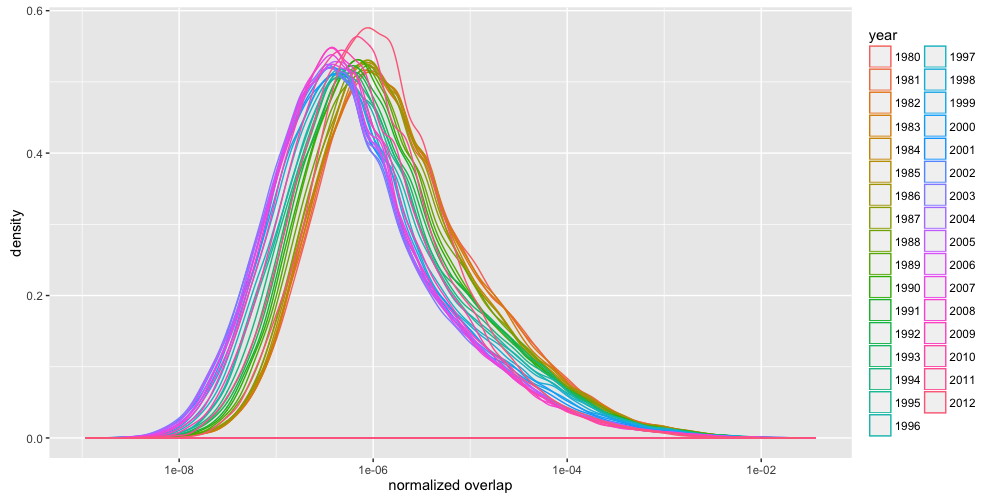
\includegraphics[width=0.49\textwidth]{figures/interov_patentnorm_all_density}
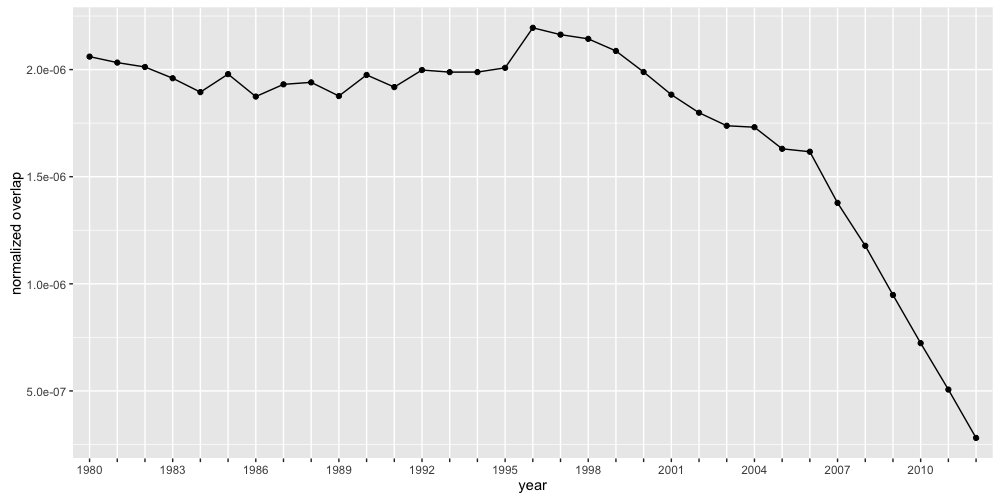
\includegraphics[width=0.49\textwidth]{figures/interov_patentnorm_all_ts}\\
\caption{Inter-classification effective overlaps (normalized by patent count)}
\end{figure}
%%%%%%%%%%%%%%%%%%%%






%%%%%%%%%%%%%%%%%%%%%%
%% Junk
%%%%%%%%%%%%%%%%%%%%%%







%Data-mining and network analysis~\cite{newman2010networks} can bring different insights.  As in science, where reflexivity is crucial and is becoming a mandatory step to build future research agendas, as e.g. in the recent analysis on 20\textsuperscript{th} century physics~\cite{Sinatra:2015yu}, the structure of technology and particularly of technological innovation necessarily involves complex patterns which understanding must have positive feedback on the economy.\par







%%%%%%%%%%%%%%%%%%%%
%%  Templates
%%%%%%%%%%%%%%%%%%%%


% For figure citations, please use "Fig." instead of "Figure".
%\begin{figure}[h]
%\caption{{\bf Figure Title first bold sentence}
%Figure Caption}
%\label{fig1}
%\end{figure}



%
%
%
%\begin{table}[!ht]
%\begin{adjustwidth}{-2.25in}{0in} % Comment out/remove adjustwidth environment if table fits in text column.
%\caption{
%{\bf Table caption Nulla mi mi, venenatis sed ipsum varius, volutpat euismod diam.}}
%\begin{tabular}{|l|l|l|l|l|l|l|l|}
%\hline
%\multicolumn{4}{|l|}{\bf Heading1} & \multicolumn{4}{|l|}{\bf Heading2}\\ \hline
%$cell1 row1$ & cell2 row 1 & cell3 row 1 & cell4 row 1 & cell5 row 1 & cell6 row 1 & cell7 row 1 & cell8 row 1\\ \hline
%$cell1 row2$ & cell2 row 2 & cell3 row 2 & cell4 row 2 & cell5 row 2 & cell6 row 2 & cell7 row 2 & cell8 row 2\\ \hline
%$cell1 row3$ & cell2 row 3 & cell3 row 3 & cell4 row 3 & cell5 row 3 & cell6 row 3 & cell7 row 3 & cell8 row 3\\ \hline
%\end{tabular}
%\begin{flushleft} Table notes Phasellus venenatis, tortor nec vestibulum mattis, massa tortor interdum felis, nec pellentesque metus tortor nec nisl. Ut ornare mauris tellus, vel dapibus arcu suscipit sed.
%\end{flushleft}
%\label{table1}
%\end{adjustwidth}
%\end{table}
%
%




%
%\subsection*{S1 Video}
%\label{S1_Video}
%{\bf Bold the first sentence.}  Maecenas convallis mauris sit amet sem ultrices gravida. Etiam eget sapien nibh. Sed ac ipsum eget enim egestas ullamcorper nec euismod ligula. Curabitur fringilla pulvinar lectus consectetur pellentesque.
%
%\subsection*{S1 Text}
%\label{S1_Text}
%{\bf Lorem Ipsum.} Maecenas convallis mauris sit amet sem ultrices gravida. Etiam eget sapien nibh. Sed ac ipsum eget enim egestas ullamcorper nec euismod ligula. Curabitur fringilla pulvinar lectus consectetur pellentesque.
%
%\subsection*{S1 Fig}
%\label{S1_Fig}
%{\bf Lorem Ipsum.} Maecenas convallis mauris sit amet sem ultrices gravida. Etiam eget sapien nibh. Sed ac ipsum eget enim egestas ullamcorper nec euismod ligula. Curabitur fringilla pulvinar lectus consectetur pellentesque.
%
%\subsection*{S2 Fig}
%\label{S2_Fig}
%{\bf Lorem Ipsum.} Maecenas convallis mauris sit amet sem ultrices gravida. Etiam eget sapien nibh. Sed ac ipsum eget enim egestas ullamcorper nec euismod ligula. Curabitur fringilla pulvinar lectus consectetur pellentesque.
%
%\subsection*{S1 Table}
%\label{S1_Table}
%{\bf Lorem Ipsum.} Maecenas convallis mauris sit amet sem ultrices gravida. Etiam eget sapien nibh. Sed ac ipsum eget enim egestas ullamcorper nec euismod ligula. Curabitur fringilla pulvinar lectus consectetur pellentesque.
%





%\begin{thebibliography}{10}
%\bibitem{bib1}
%Devaraju P, Gulati R, Antony PT, Mithun CB, Negi VS. Susceptibility to SLE in South Indian Tamils may be influenced by genetic selection pressure on TLR2 and TLR9 genes. Mol Immunol. 2014 Nov 22. pii: S0161-5890(14)00313-7. doi: 10.1016/j.molimm.2014.11.005

%\bibitem{bib2}
%Huynen MMTE, Martens P, Hilderlink HBM. The health impacts of globalisation: a conceptual framework. Global Health. 2005;1: 14. Available: http://www.globalizationandhealth.com/content/1/1/14.

%\end{thebibliography}







\end{document}
